\chapter{Province du Guizhou}
\section*{16 octobre 2015}
De Leshan je me dirige vers le sud ouest et la province du Guizhou. \newline
 Beaucoup de production de fruits dans le coin, des dizaines de stands vendent les pomelos \newline
 \newline
\centerline{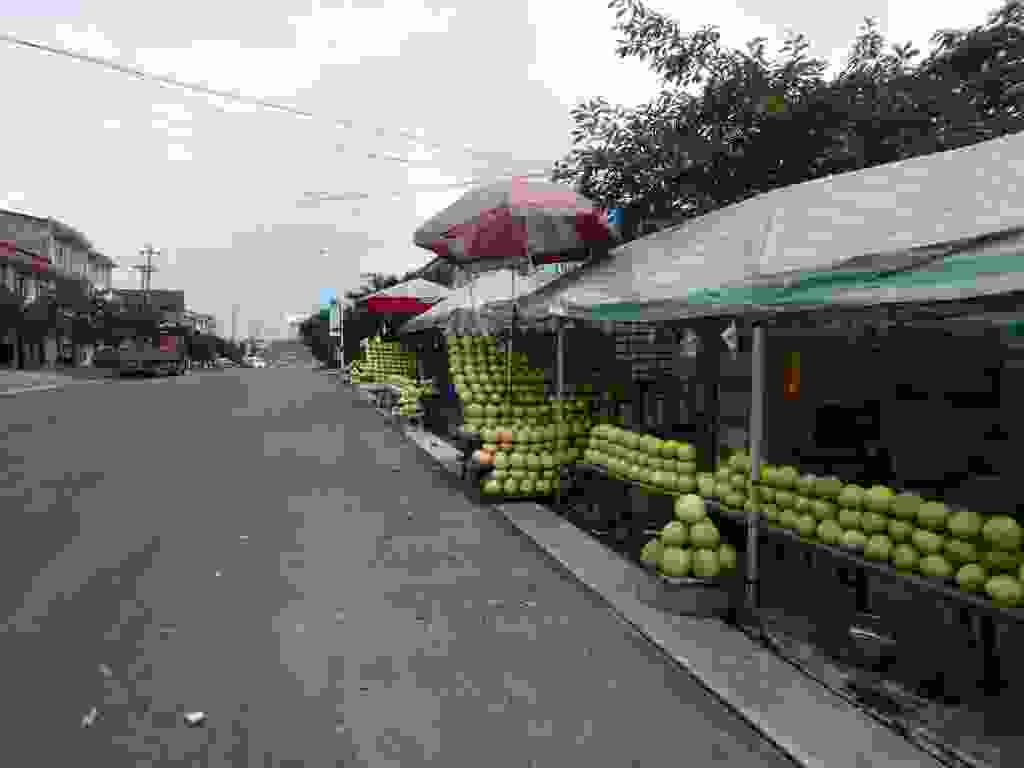
\includegraphics[height=90mm]{../wp-content/uploads/2015/10/wpid-p9300036-1024x768.jpg} } 
 \newline
 \newline
\centerline{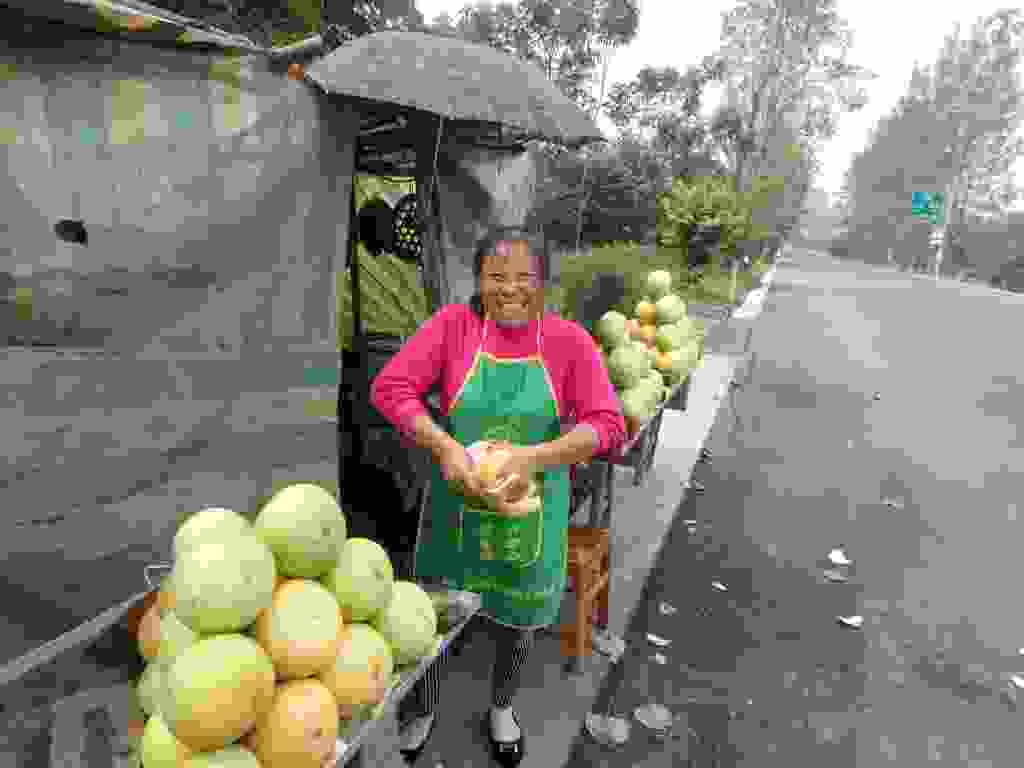
\includegraphics[height=90mm]{../wp-content/uploads/2015/10/wpid-p9300035-1024x768.jpg} } 
 \newline
 Je m'arrête dans les petits restos, la cuisine est à l'extérieur \newline
 \newline
\centerline{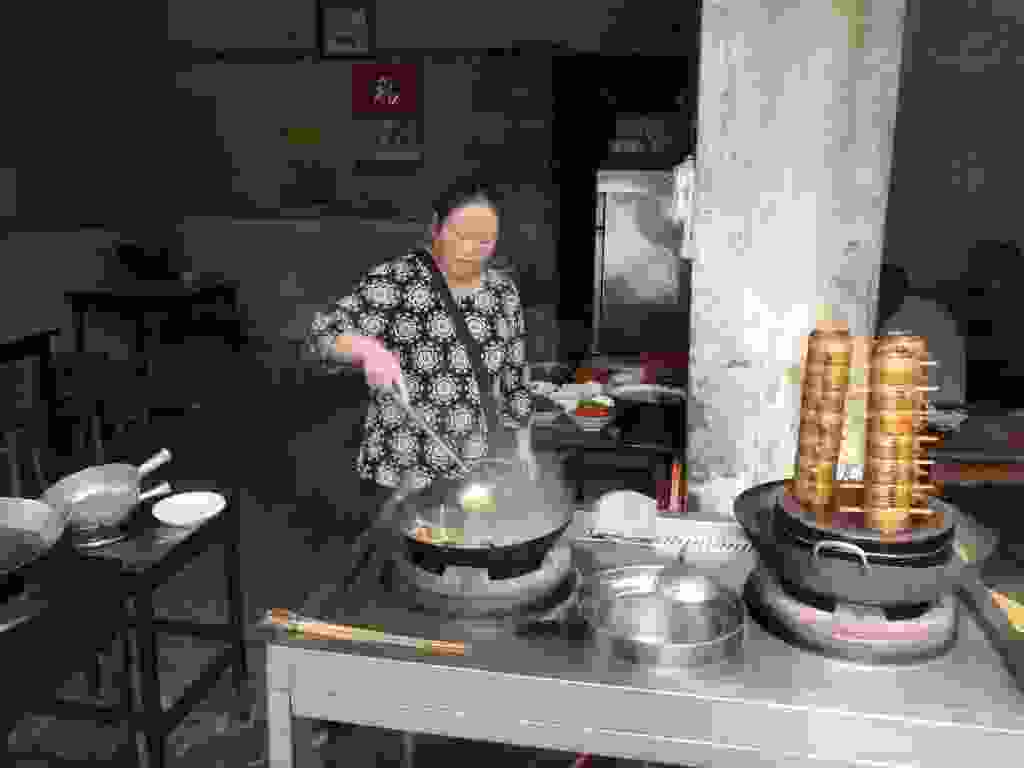
\includegraphics[height=90mm]{../wp-content/uploads/2015/10/wpid-p9300038-1024x768.jpg} } 
 \newline
 \newline
\centerline{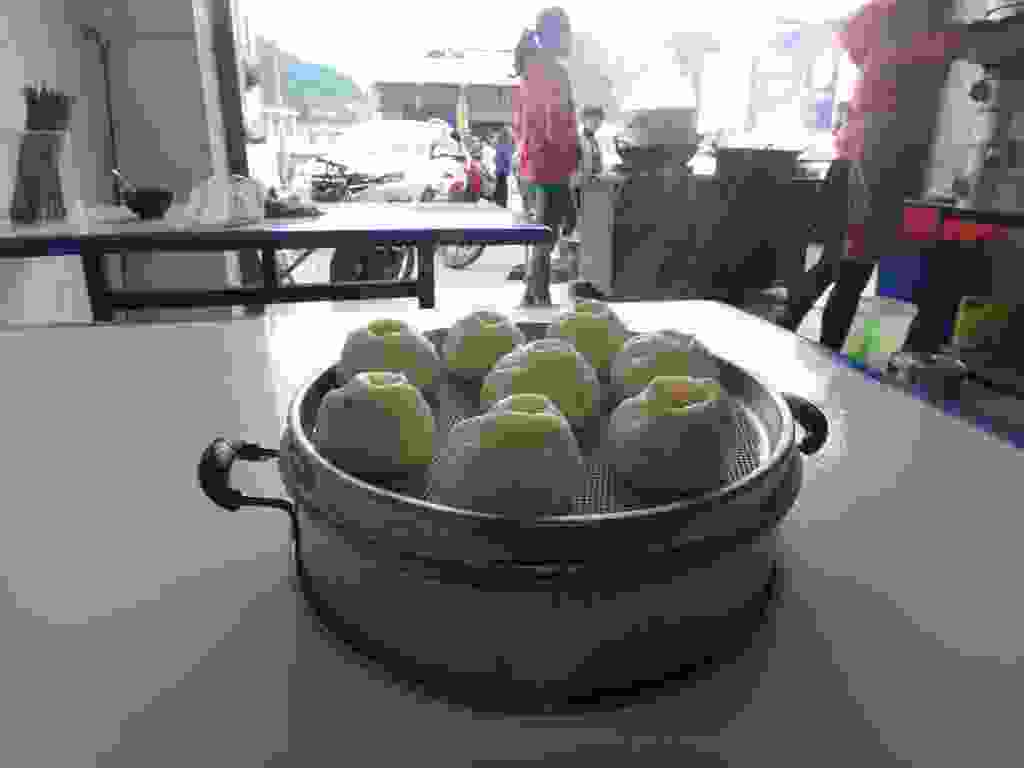
\includegraphics[height=90mm]{../wp-content/uploads/2015/10/wpid-pa040102-1024x768.jpg} } 
 \newline
 Les villes sont rarement les mêmes : certaines sont très propres et modernes, d'autres plus industrielles et moins agréables. \newline
 \newline
\centerline{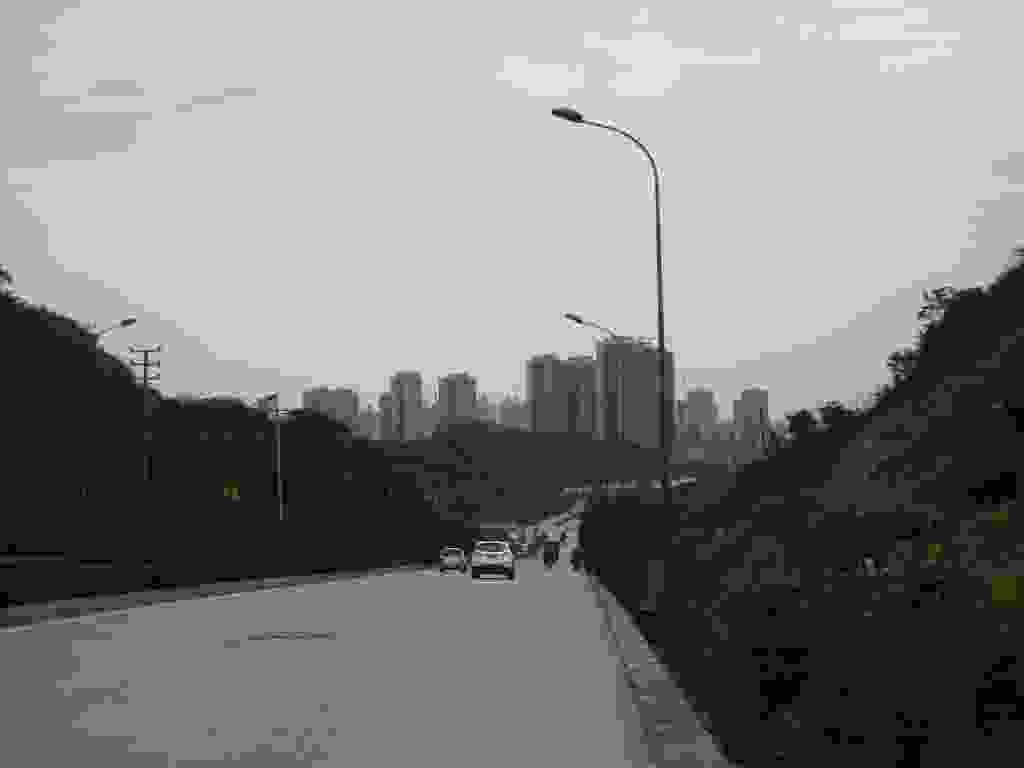
\includegraphics[height=90mm]{../wp-content/uploads/2015/10/wpid-pa010051-1024x768.jpg} } 
 \newline
 \newline
\centerline{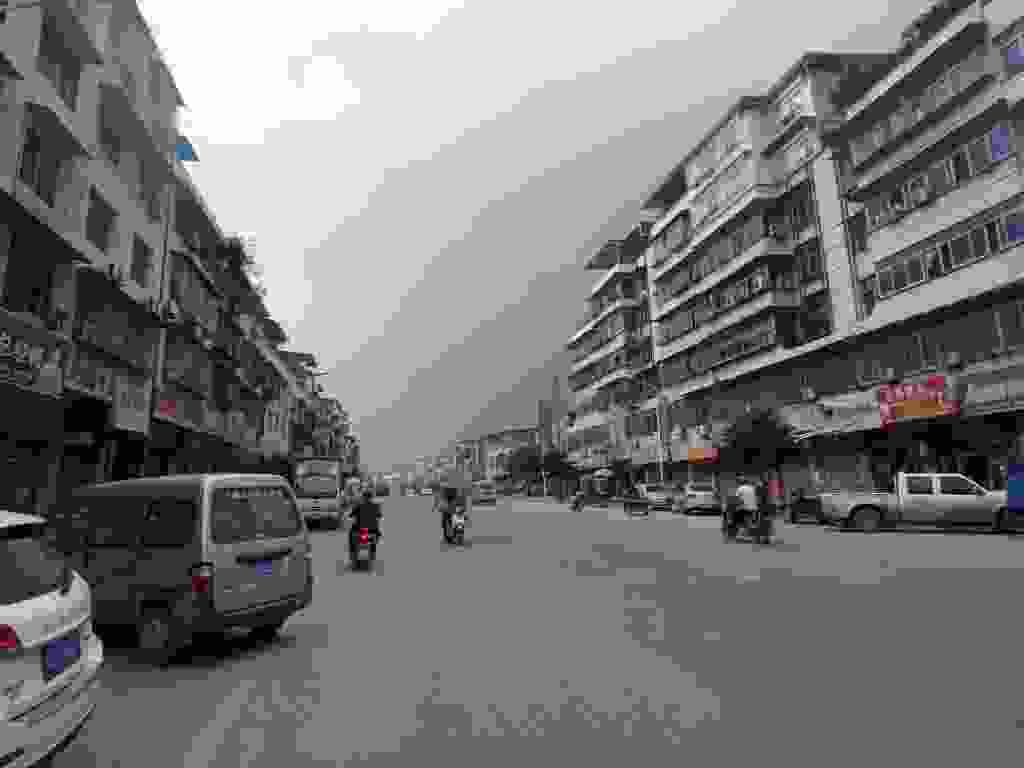
\includegraphics[height=90mm]{../wp-content/uploads/2015/10/P9300043-1024x768.jpg} } 
 \newline
 \newline
\centerline{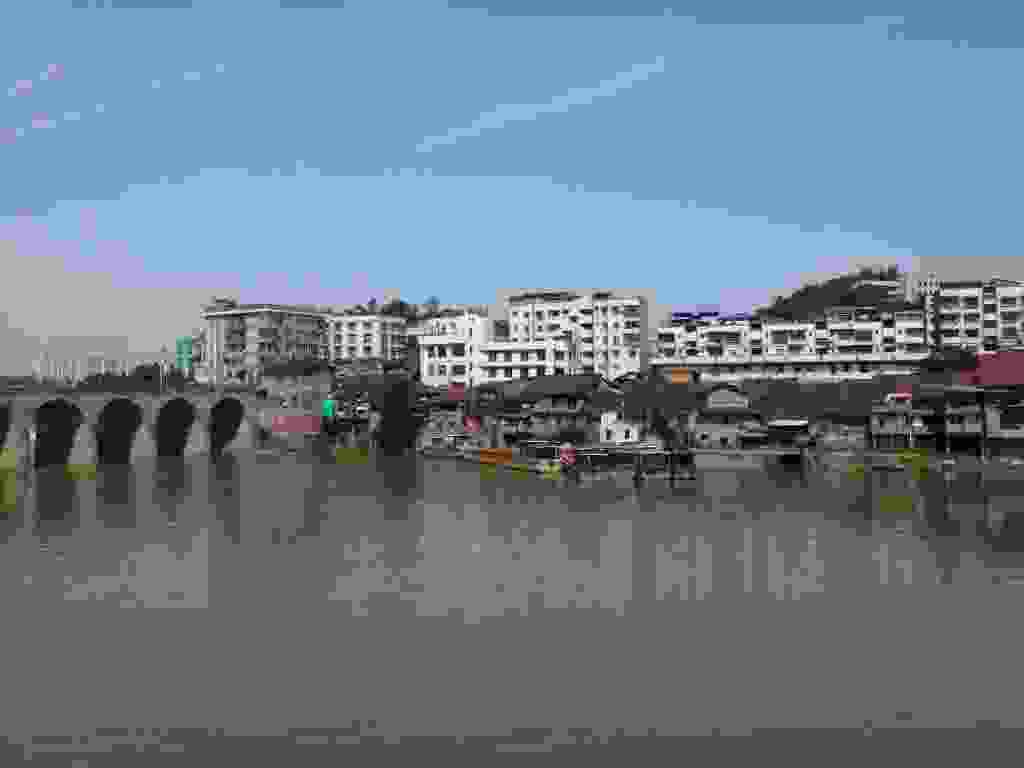
\includegraphics[height=90mm]{../wp-content/uploads/2015/10/wpid-pa010052-1024x768.jpg} } 
 \newline
 \newline
\centerline{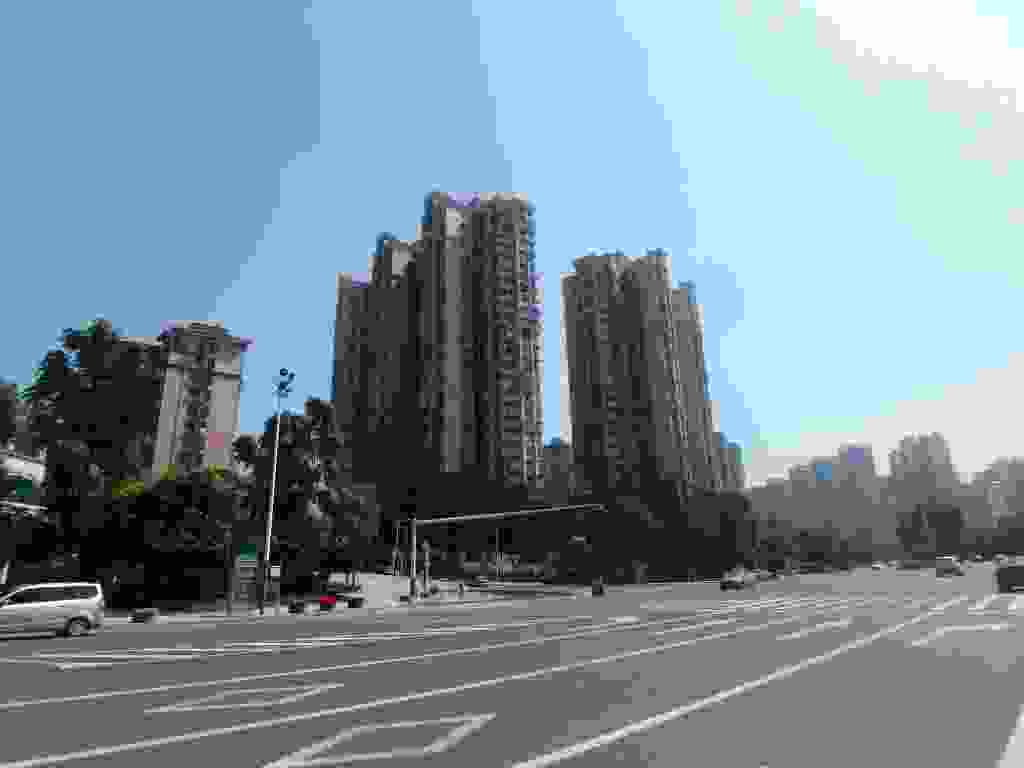
\includegraphics[height=90mm]{../wp-content/uploads/2015/10/wpid-pa020077-1024x768.jpg} } 
 \newline
 \newline
\centerline{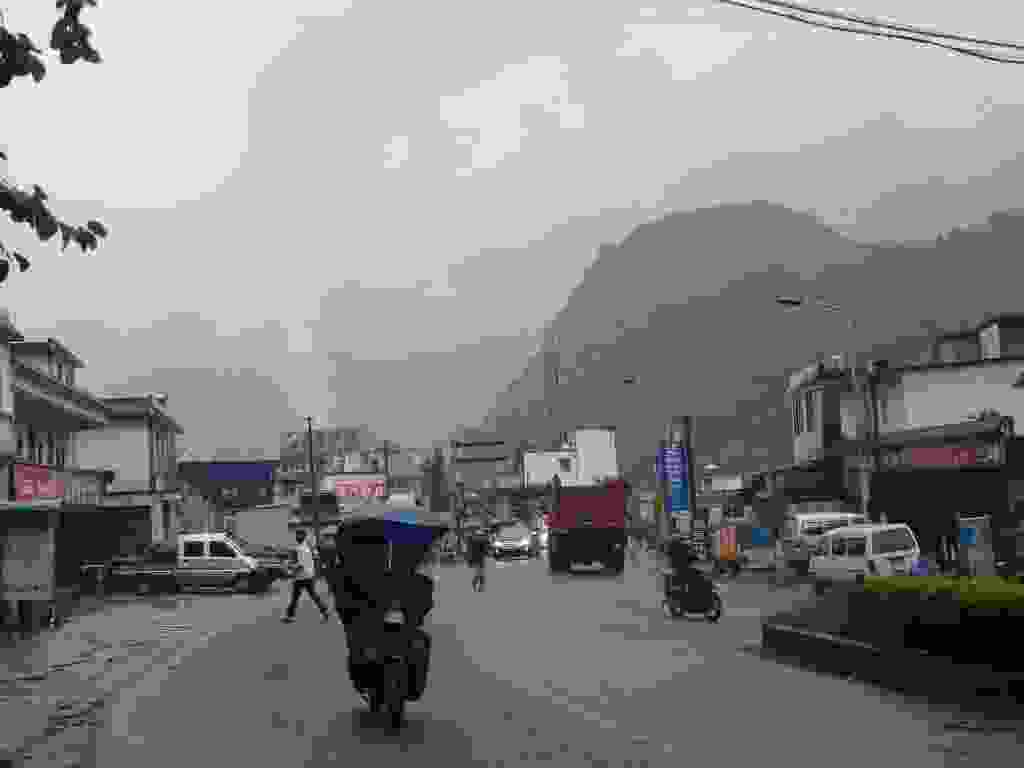
\includegraphics[height=90mm]{../wp-content/uploads/2015/10/wpid-pa040097-1024x768.jpg} } 
 \newline
 Un soir je termine dans le village de Zaozhua, il reste quelques ruelles au centre avec des maisons traditionnelles bien conservées et pas transformées en parc d'attraction touristique, rare en Chine \newline
 \newline
\centerline{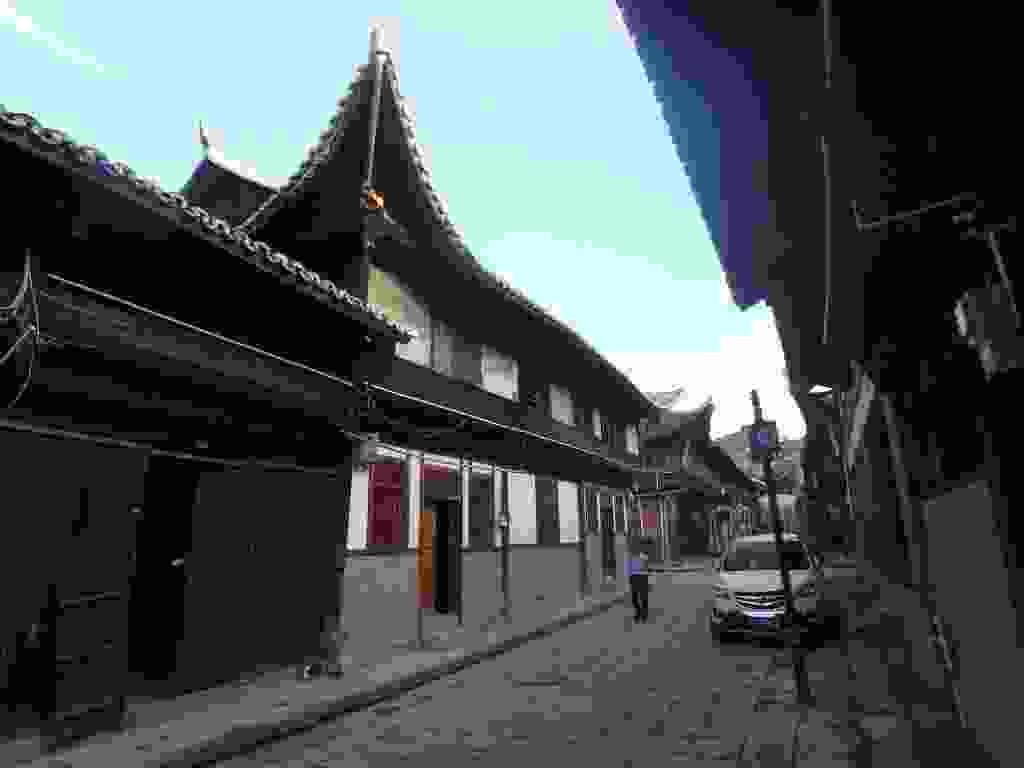
\includegraphics[height=90mm]{../wp-content/uploads/2015/10/wpid-pa010061-1024x768.jpg} } 
 \newline
 \newline
\centerline{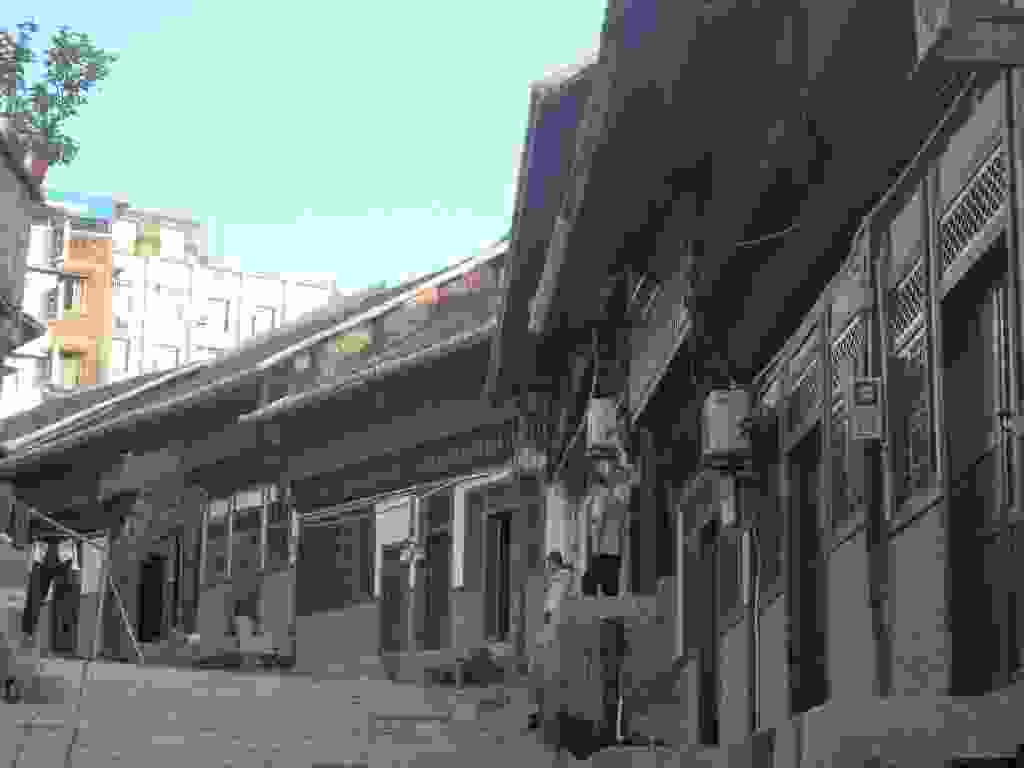
\includegraphics[height=90mm]{../wp-content/uploads/2015/10/wpid-pa010062-1024x768.jpg} } 
 \newline
 \newline
\centerline{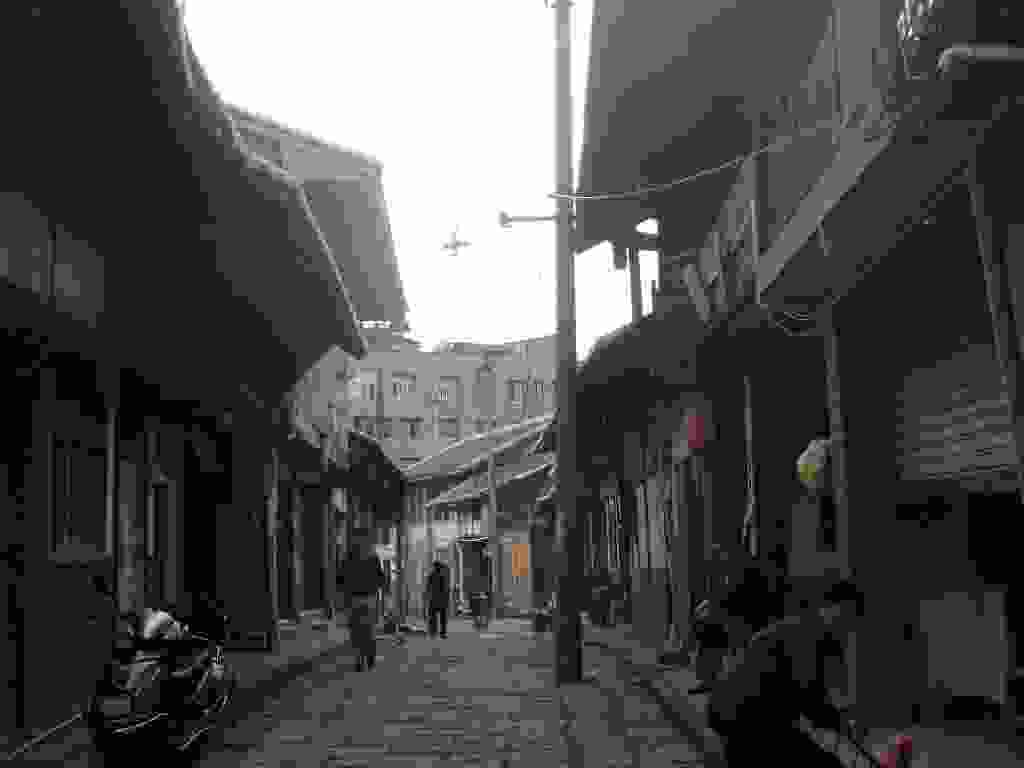
\includegraphics[height=90mm]{../wp-content/uploads/2015/10/wpid-pa010067-1024x768.jpg} } 
 \newline
 Au moment de trouver un hôtel ça se complique : pour recevoir les étrangers les hôtels doivent avoir une licence spéciale. Les 3 premiers hôtels qu'on m'indique me refusent. \newline
 Finalement un groupe de jeunes m'aide à en trouver un autre qui accepte, même s'il n'a pas l'air specialement agréé \newline
 \newline
\centerline{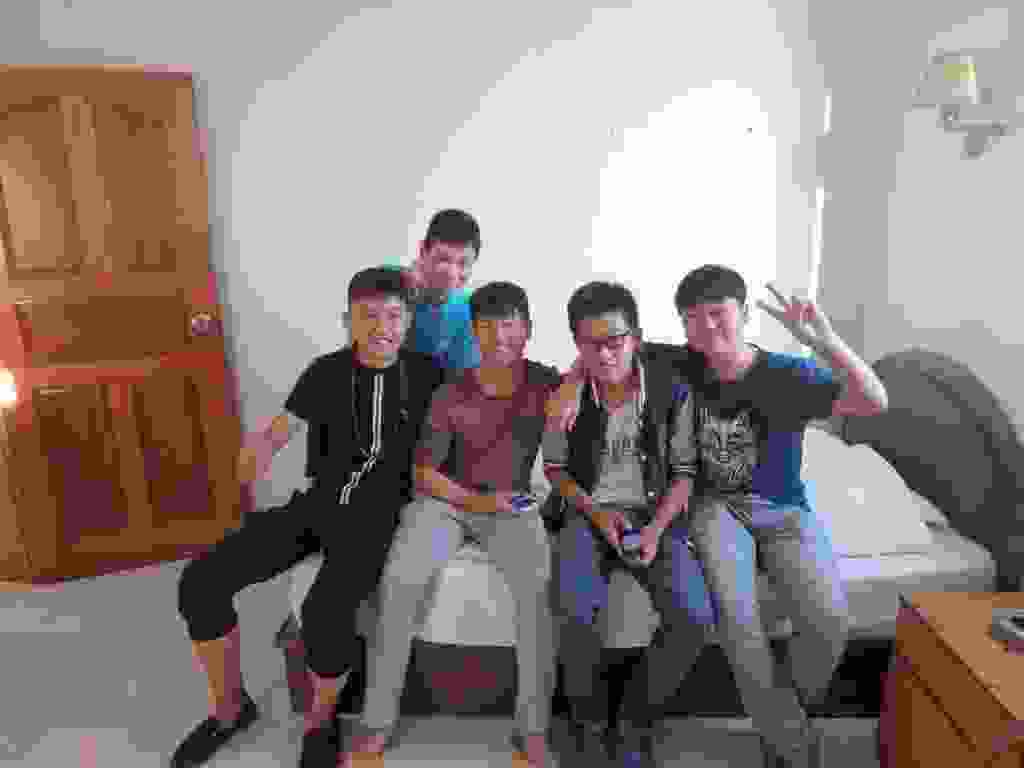
\includegraphics[height=90mm]{../wp-content/uploads/2015/10/wpid-pa010057-1024x768.jpg} } 
 \newline
 Je sors sur la place du village où des gens viennent danser une chorégraphie devant un petit haut parleur. Un peu plus tard un deuxième groupe se lance à côté avec une musique différente ! \newline
 \newline
\centerline{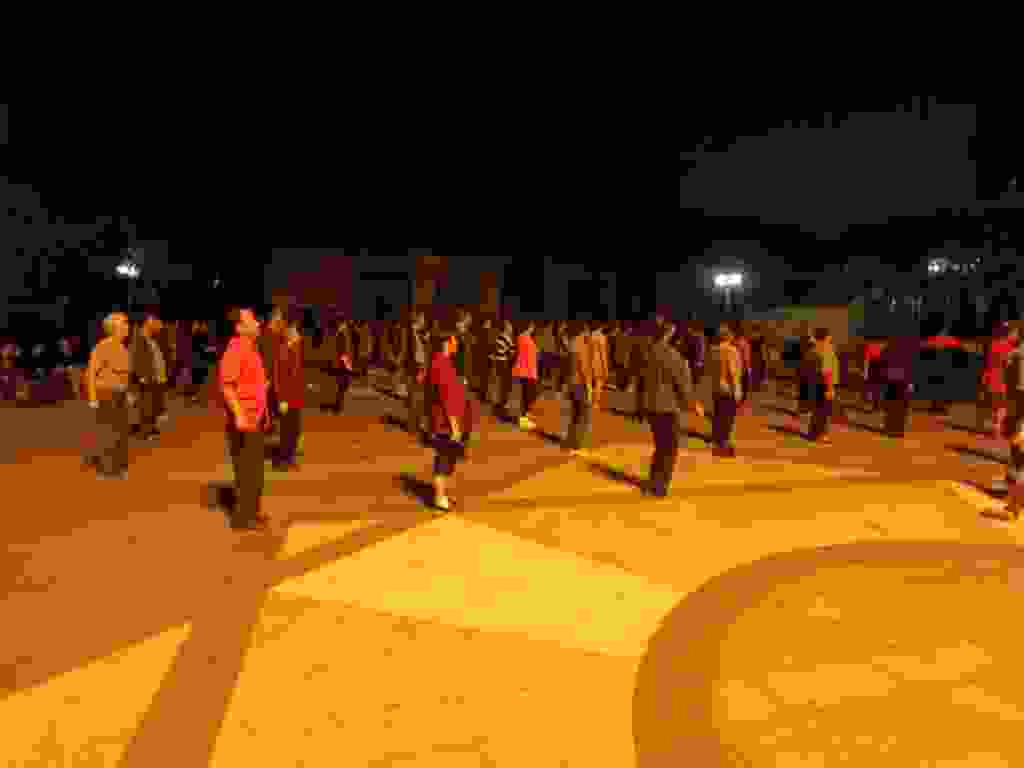
\includegraphics[height=90mm]{../wp-content/uploads/2015/10/wpid-pa010074-1024x768.jpg} } 
 \newline
 Quand je reviens à l'hôtel plus tard, la police m'attend et me dit que je ne peux pas rester ici. Une voiture de police m'escorte jusqu'à un autre hôtel, pas vraiment différent mais autorisé… \newline
 Le lendemain, je suis stoppé quelques minutes par un accident qui a provoqué un gros bouchon, les gens sont descendu voir ce qui se passait. \newline
 \newline
\centerline{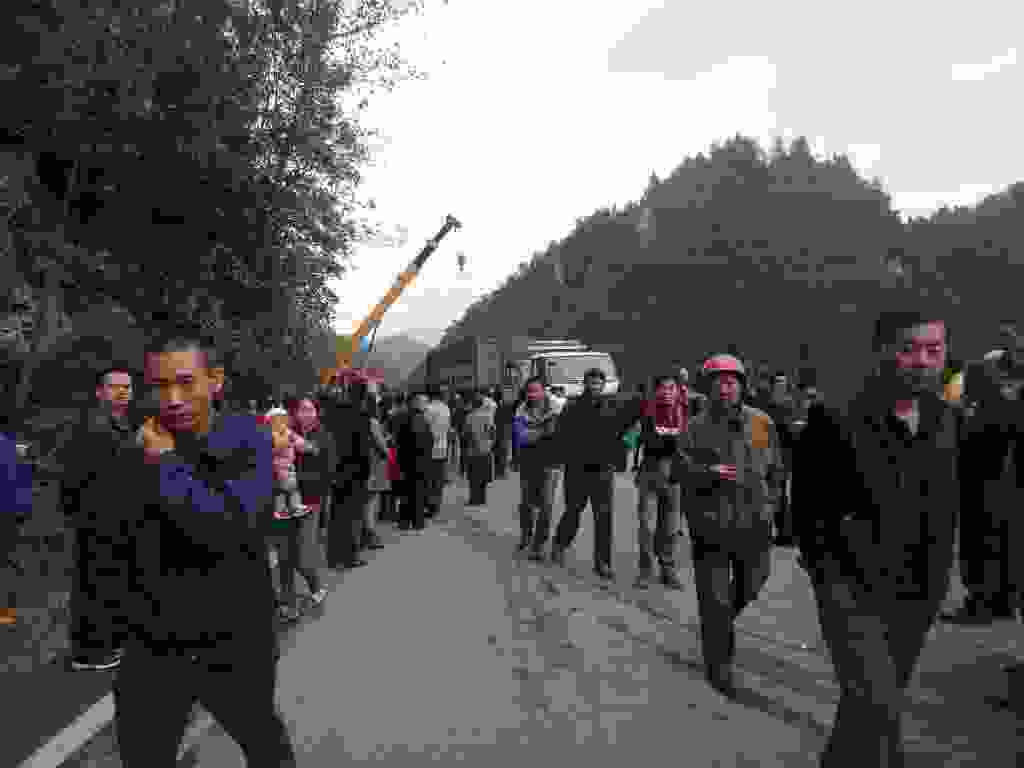
\includegraphics[height=90mm]{../wp-content/uploads/2015/10/wpid-pa040103-1024x768.jpg} } 
 \newline
 Apiculteur au bord de la route, miel directement du producteur \newline
 \newline
\centerline{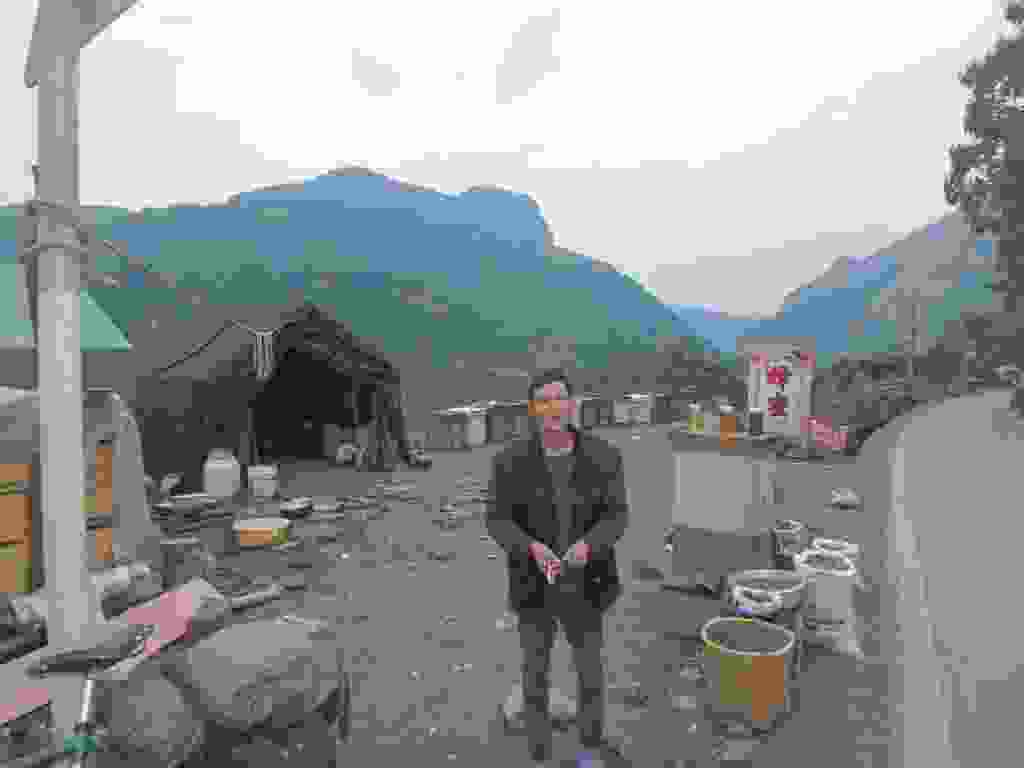
\includegraphics[height=90mm]{../wp-content/uploads/2015/10/wpid-pa040106-1024x768.jpg} } 
 \newline
 La route longe parfois une rivière, le plat ne dure jamais longtemps \newline
 \newline
\centerline{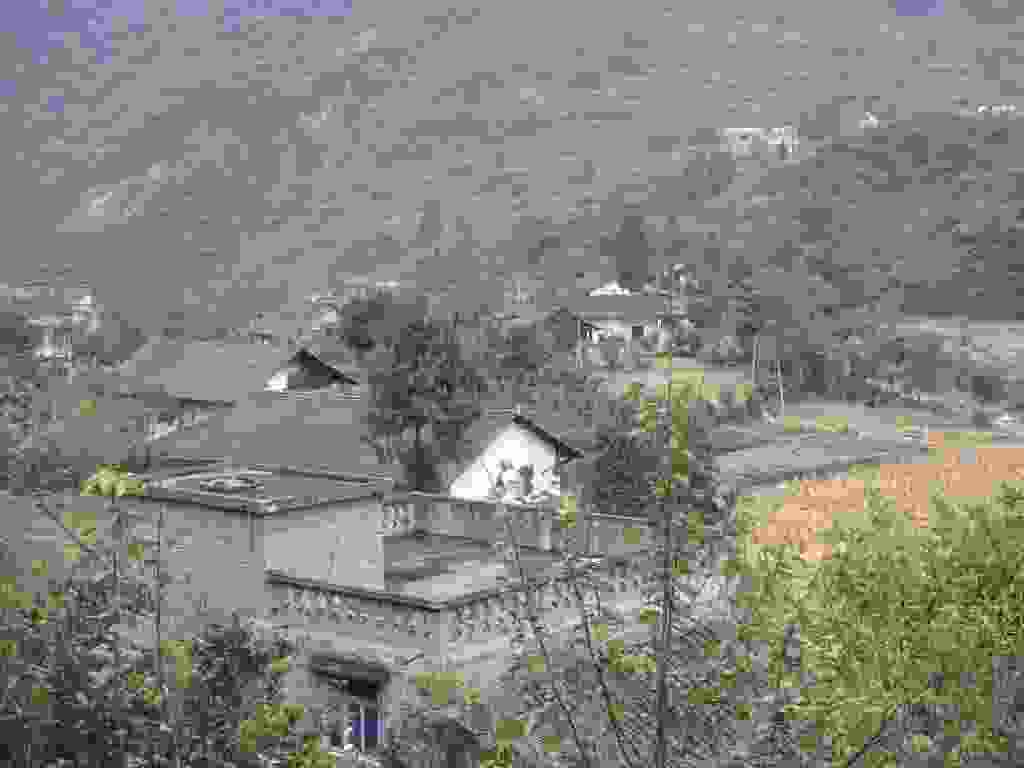
\includegraphics[height=90mm]{../wp-content/uploads/2015/10/wpid-pa040107-1024x768.jpg} } 
 \newline
 \newline
\centerline{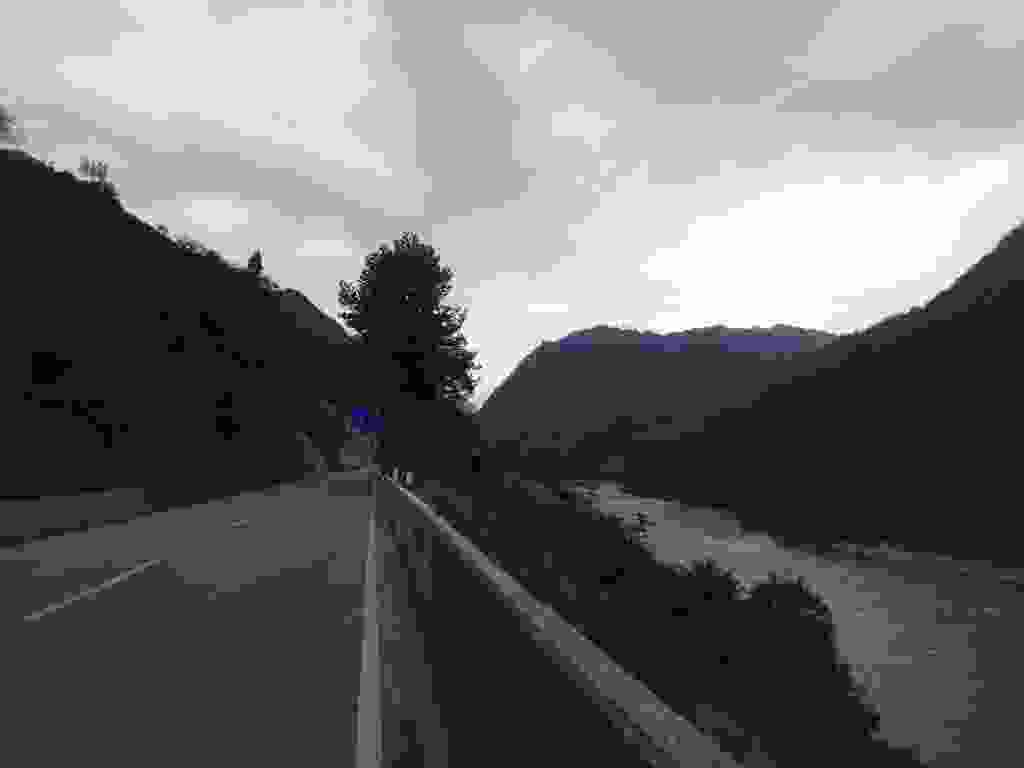
\includegraphics[height=90mm]{../wp-content/uploads/2015/10/wpid-pa040110-1024x768.jpg} } 
 \newline
 J'emprunte une autoroute sur une centaine de km, les viaducs permettent de profiter de vues magnifiques \newline
 \newline
\centerline{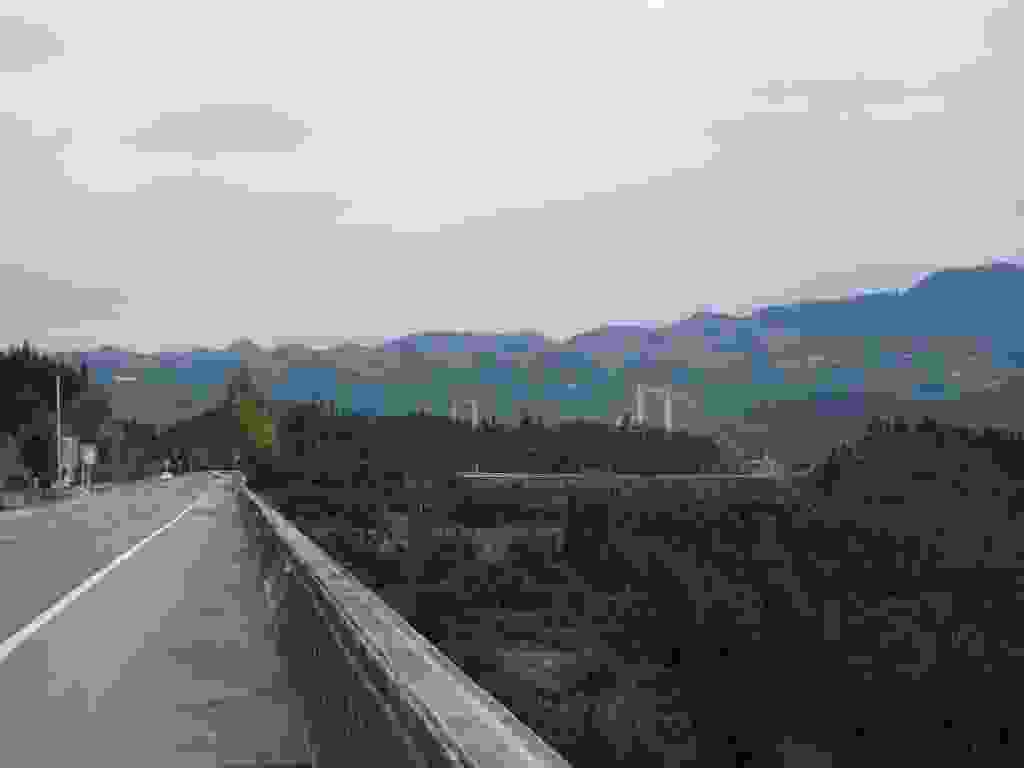
\includegraphics[height=90mm]{../wp-content/uploads/2015/10/wpid-pa060140-1024x768.jpg} } 
 \newline
 \newline
\centerline{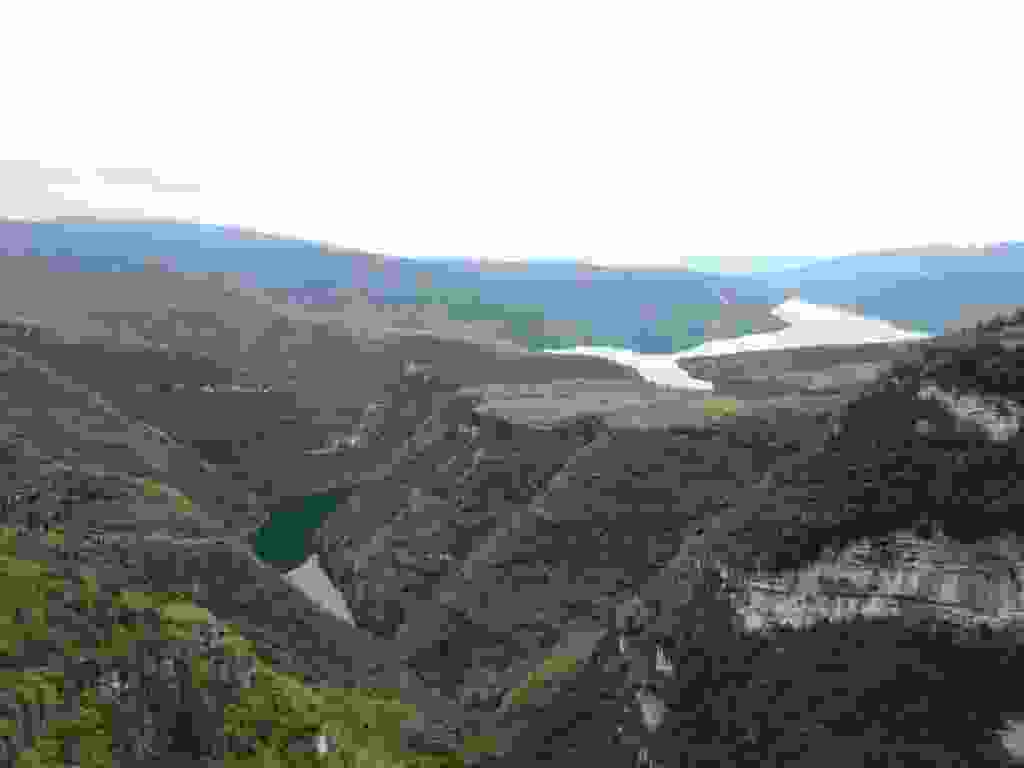
\includegraphics[height=90mm]{../wp-content/uploads/2015/10/wpid-pa060141-1024x768.jpg} } 
 \newline
 \newline
\centerline{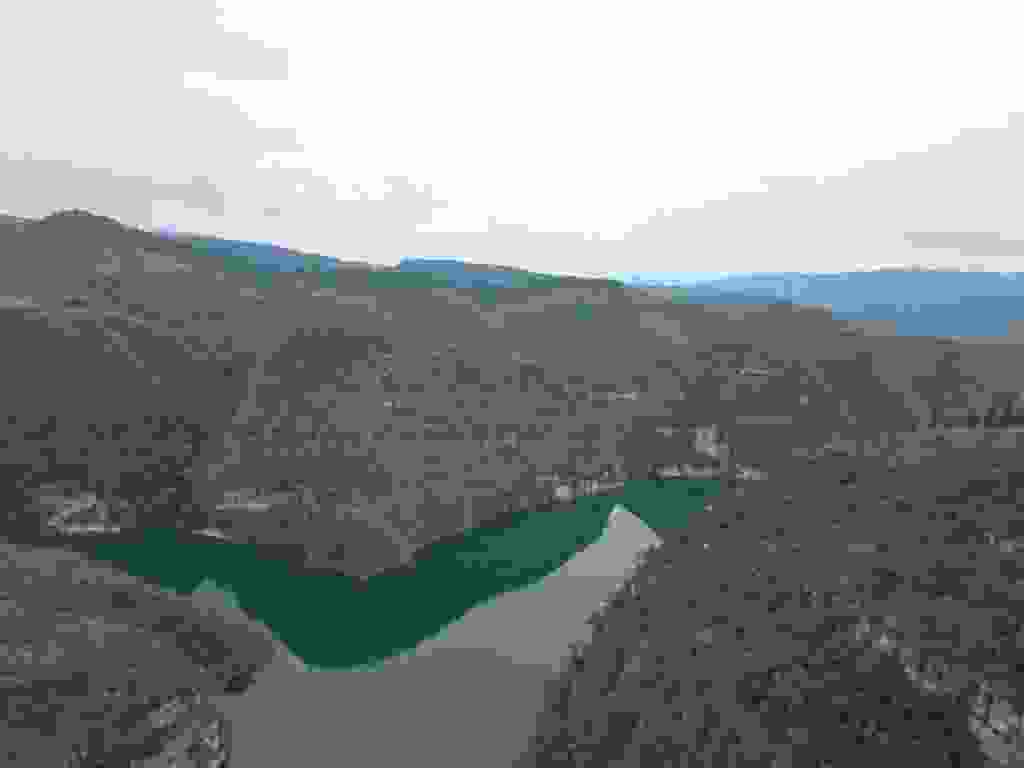
\includegraphics[height=90mm]{../wp-content/uploads/2015/10/wpid-pa060143-1024x768.jpg} } 
 \newline
 \newline
\centerline{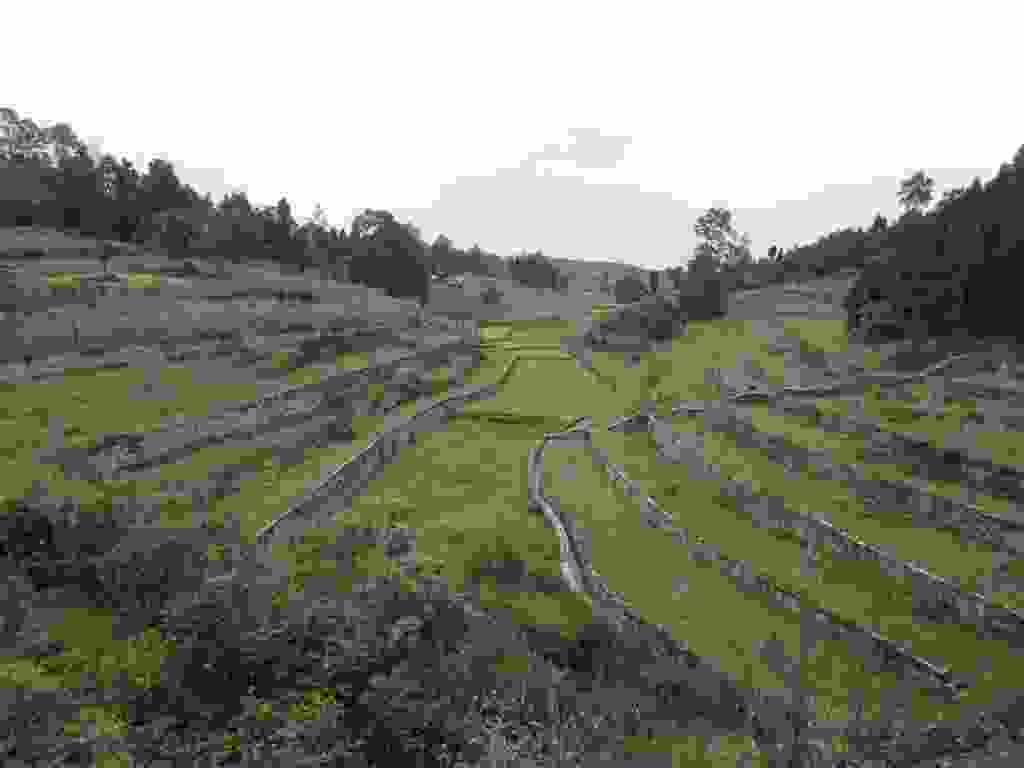
\includegraphics[height=90mm]{../wp-content/uploads/2015/10/wpid-pa060147-1024x768.jpg} } 
 \newline
 \newline
\centerline{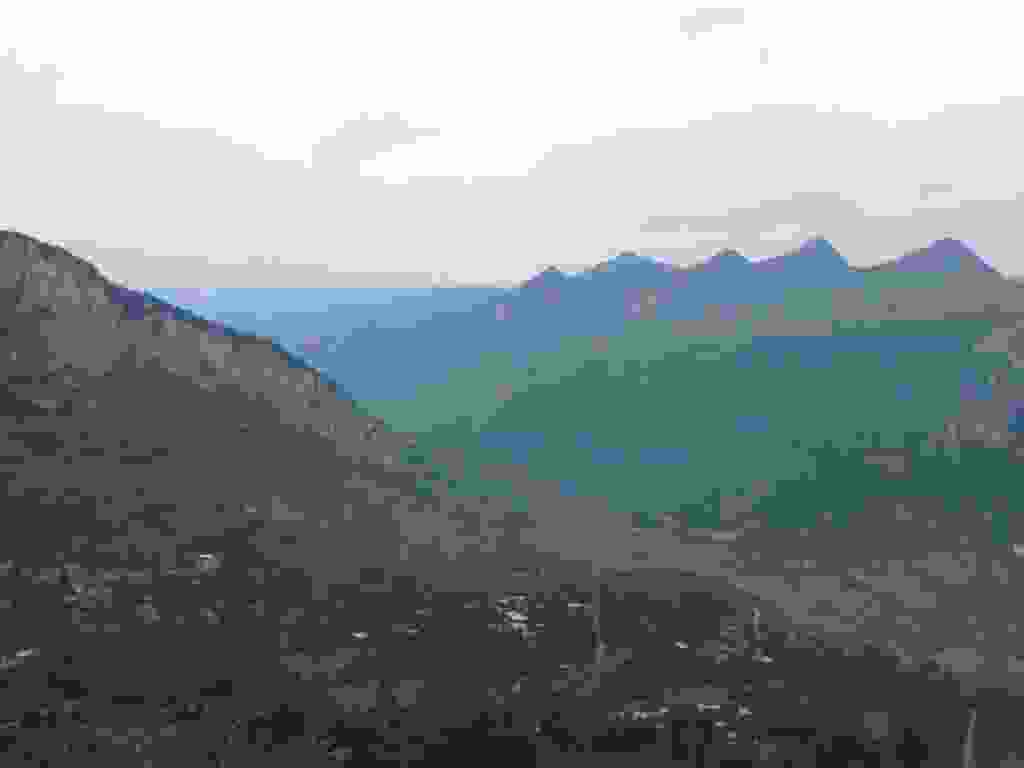
\includegraphics[height=90mm]{../wp-content/uploads/2015/10/wpid-pa070153-1024x768.jpg} } 
 \newline
 \newline
\centerline{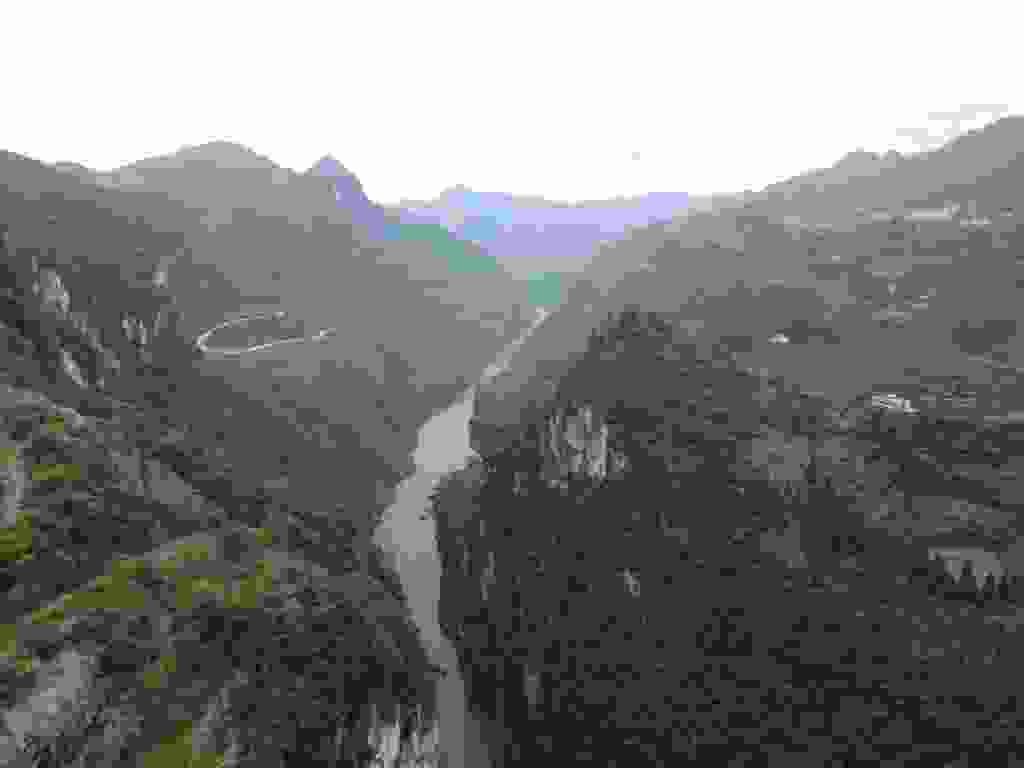
\includegraphics[height=90mm]{../wp-content/uploads/2015/10/wpid-pa070155-1024x768.jpg} } 
 \newline
 Je fais les derniers km avant Guiyang avec un groupe de cyclistes chinois. Ils m'ont invité à partager leur repas alors que je passais devant un resto \newline
 \newline
\centerline{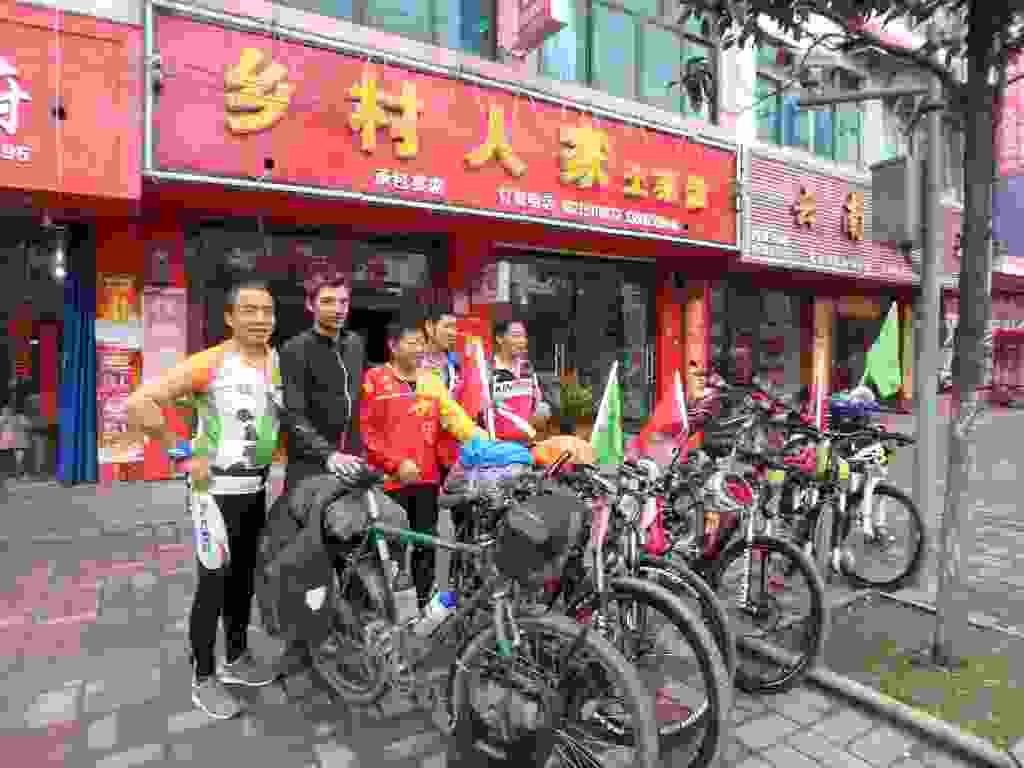
\includegraphics[height=90mm]{../wp-content/uploads/2015/10/wpid-pa070158-1024x768.jpg} } 
 \newline
 Guiyang est la capitale du Guizhou \newline
 \newline
\centerline{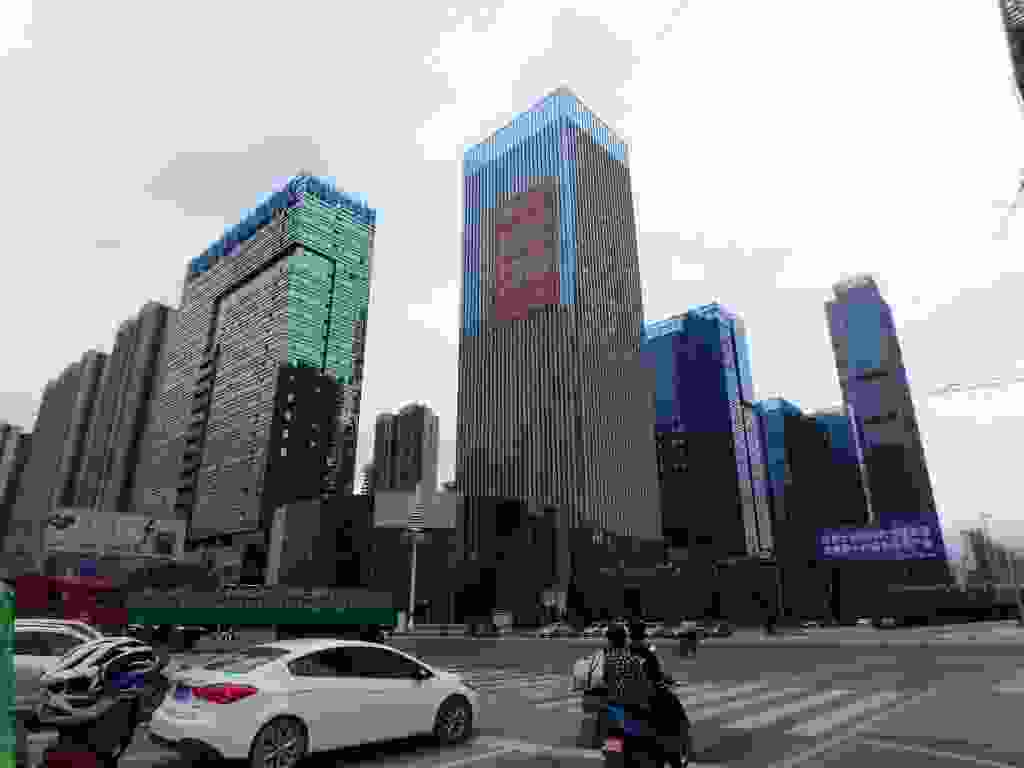
\includegraphics[height=90mm]{../wp-content/uploads/2015/10/PA070162-1024x768.jpg} } 
 \newline
 \newline
\centerline{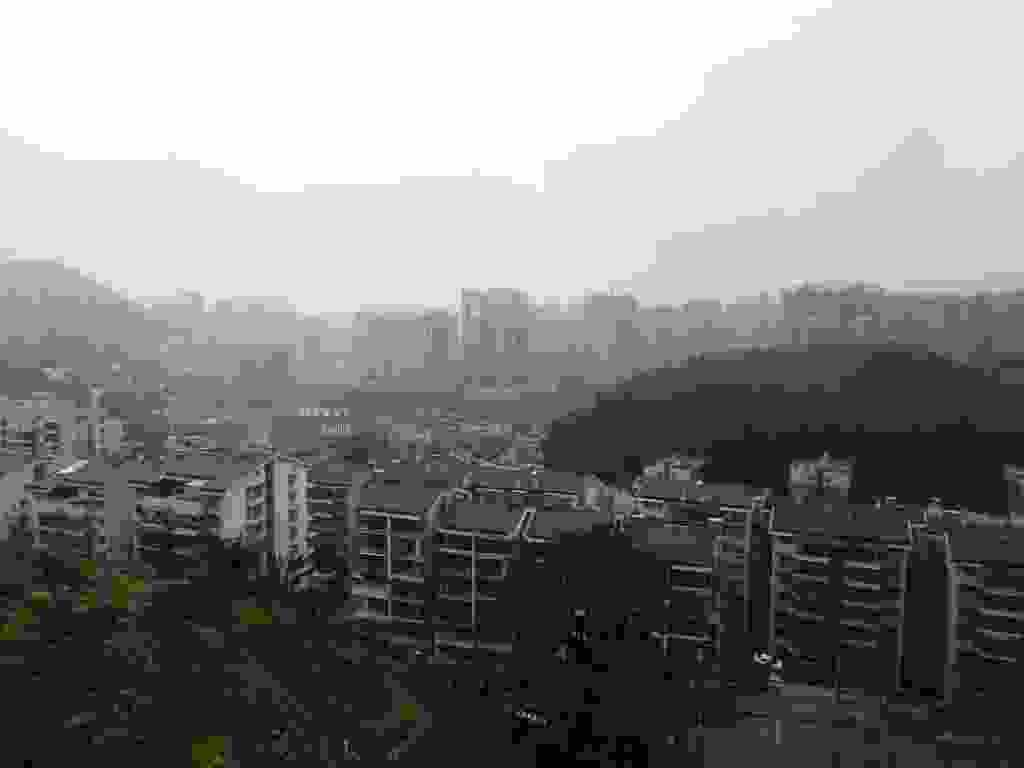
\includegraphics[height=90mm]{../wp-content/uploads/2015/10/PA090167-1024x768.jpg} } 
 \newline
 Maria et Ivan, des warmshowers espagnols très sympa m'y ont accueilli pendant 2 jours \newline
 \newline
\centerline{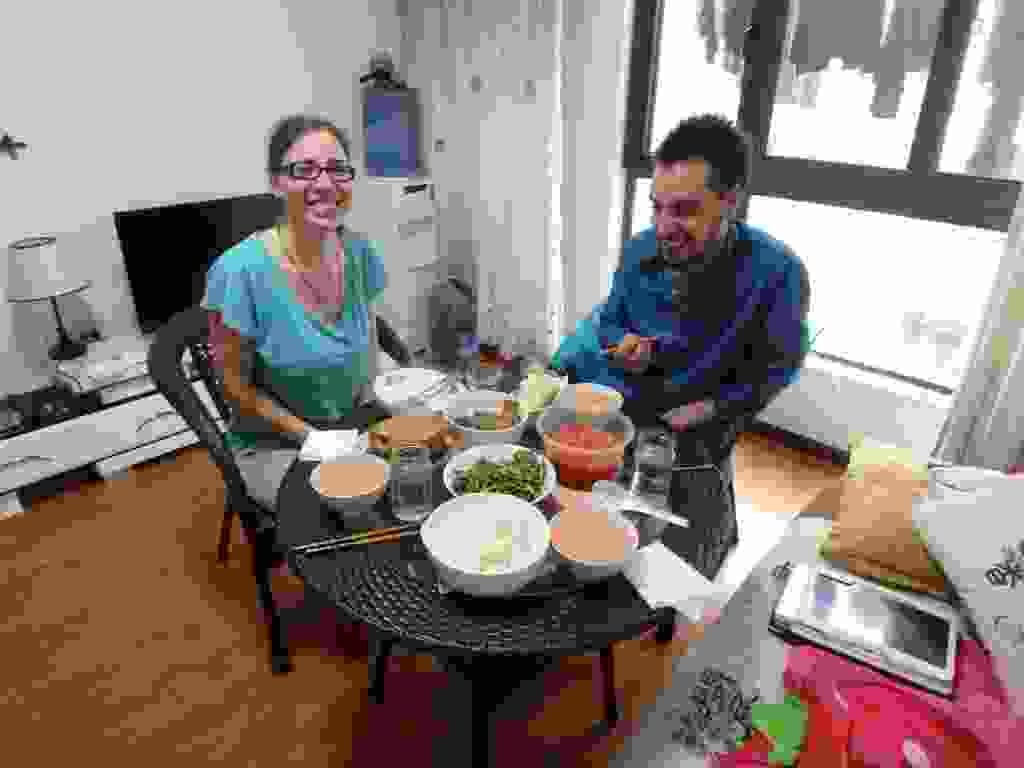
\includegraphics[height=90mm]{../wp-content/uploads/2015/10/PA080163-1024x768.jpg} } 
 \newline
 Je repars sur une route en travaux en mauvais état \newline
 \newline
\centerline{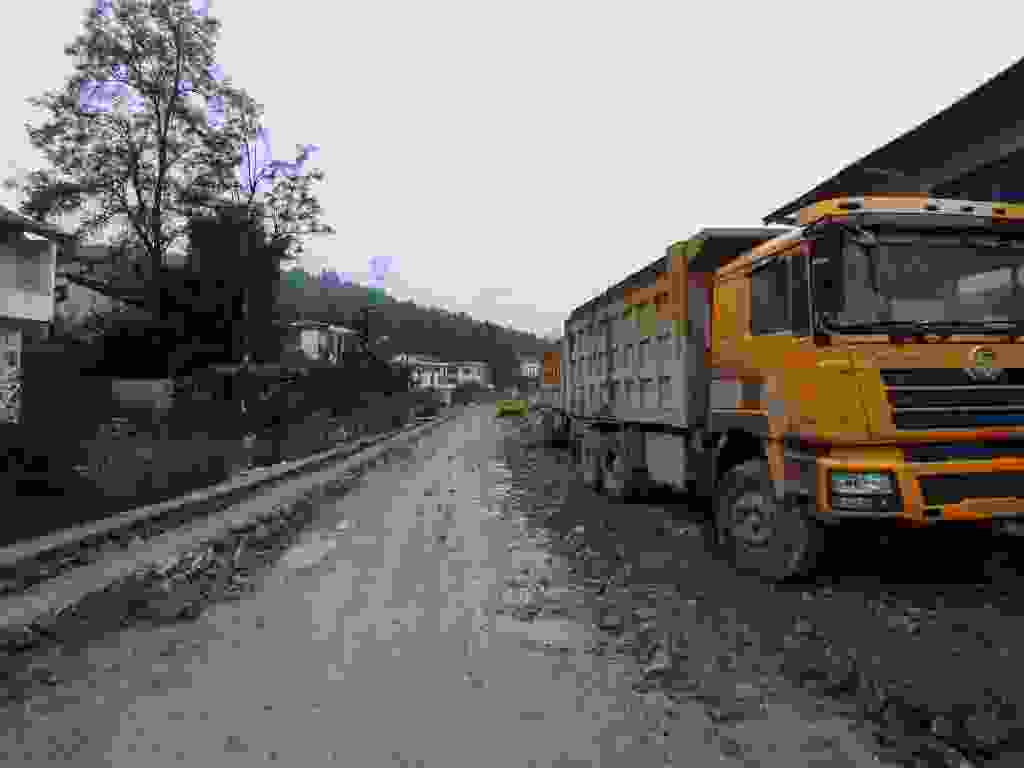
\includegraphics[height=90mm]{../wp-content/uploads/2015/10/PA090170-1024x768.jpg} } 
 \newline
 \newline
\centerline{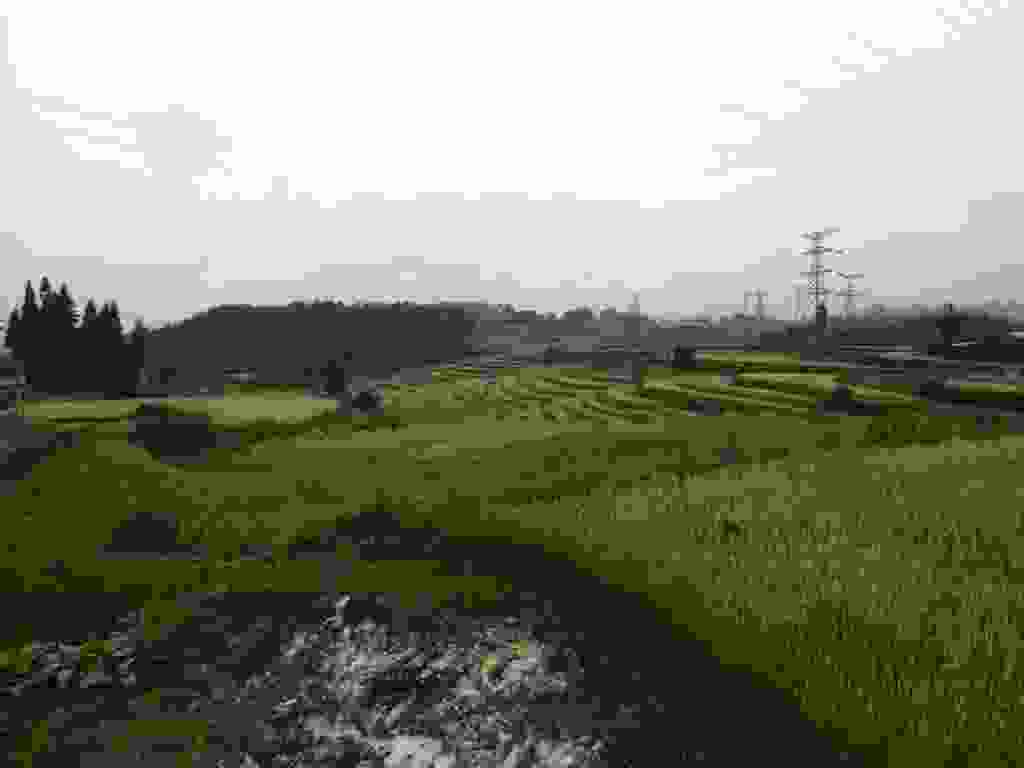
\includegraphics[height=90mm]{../wp-content/uploads/2015/10/PA090172-1024x768.jpg} } 
 \newline
 Alors que je m'arrête pour chercher un hôtel à Guiding, je m'aperçois que j'ai perdu le sac a dos que je fixe à l'arrière du vélo. Je fais demi tour en espérant le retrouver. Quelques km et je tombe sur la protection de pluie du sac mais sans le sac : quelqu'un s'est servi apparemment. \newline
 Du coup je fais appel à la police, on ne sait jamais. Ils essayent de m'aider, on revient sur les lieux, ils visionnent des cameras de surveillance, on ne trouve pas le sac. En tout cas je peux dire que la police chinoise est sympa, ils m'ont offert à manger et m'ont aidé le lendemain à racheter des objets perdus. \newline
 \newline
\centerline{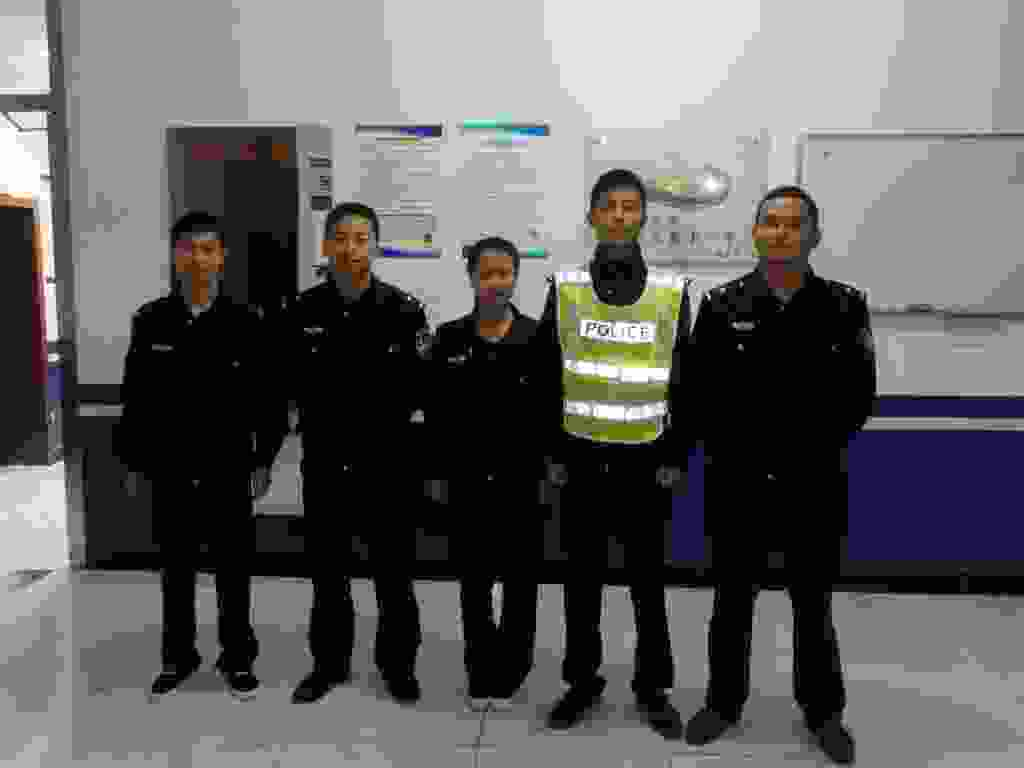
\includegraphics[height=90mm]{../wp-content/uploads/2015/10/PA090173-1024x768.jpg} } 
 \newline
 \newline
\centerline{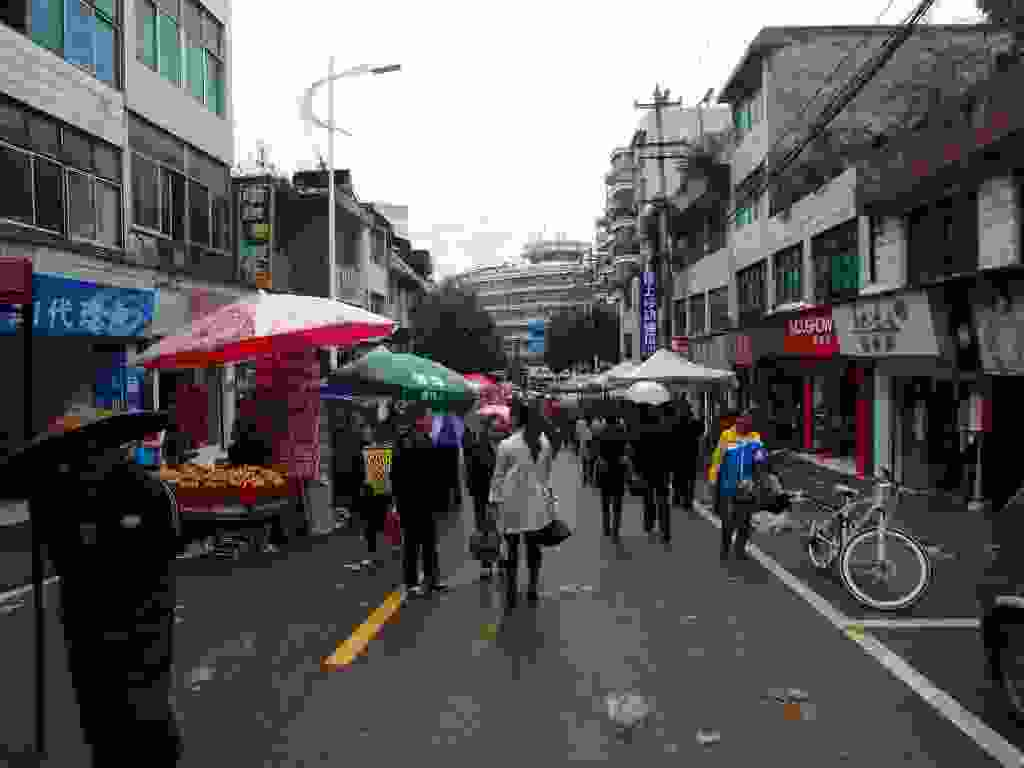
\includegraphics[height=90mm]{../wp-content/uploads/2015/10/PA100177-1024x768.jpg} } 
 \newline
 Je continue un peu plus léger, j'apprécie quelques journées ensoleillées \newline
 \newline
\centerline{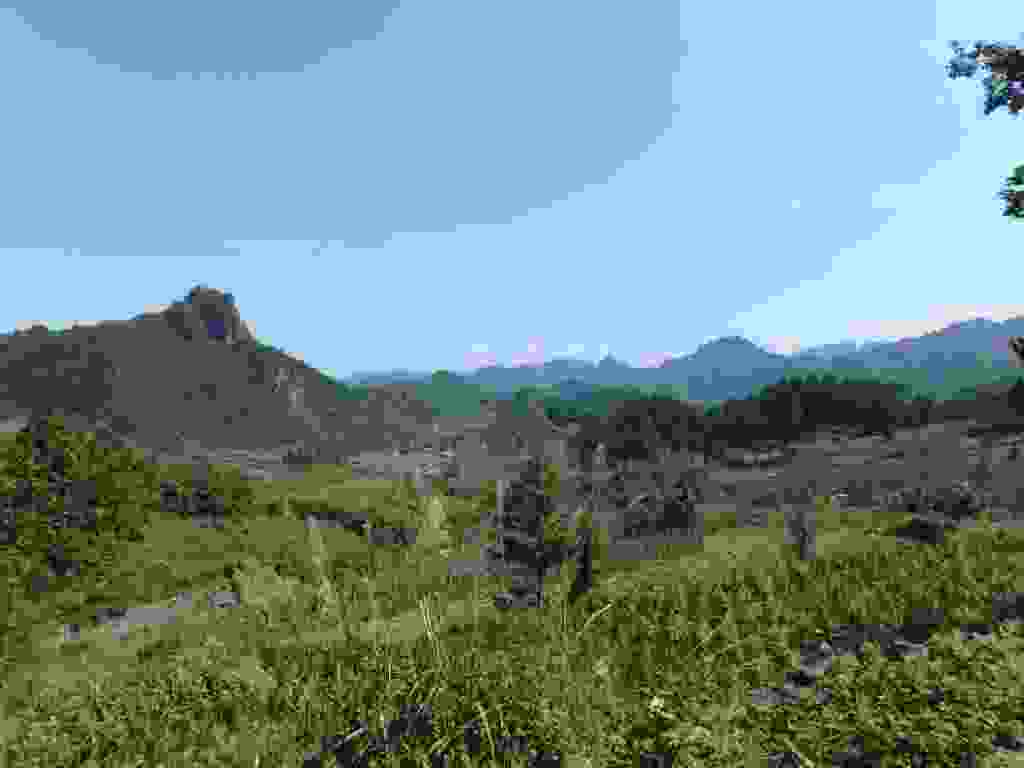
\includegraphics[height=90mm]{../wp-content/uploads/2015/10/PA110185-1024x768.jpg} } 
 \newline
 \newline
\centerline{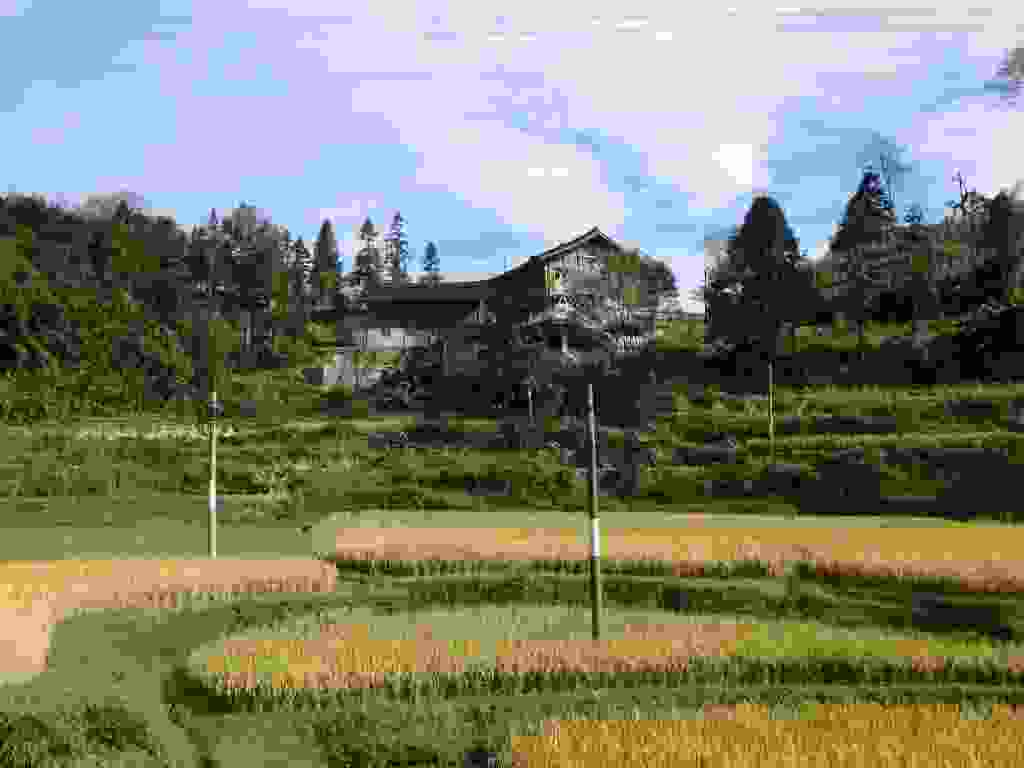
\includegraphics[height=90mm]{../wp-content/uploads/2015/10/PA120195-1024x768.jpg} } 
 \newline
 \newline
\centerline{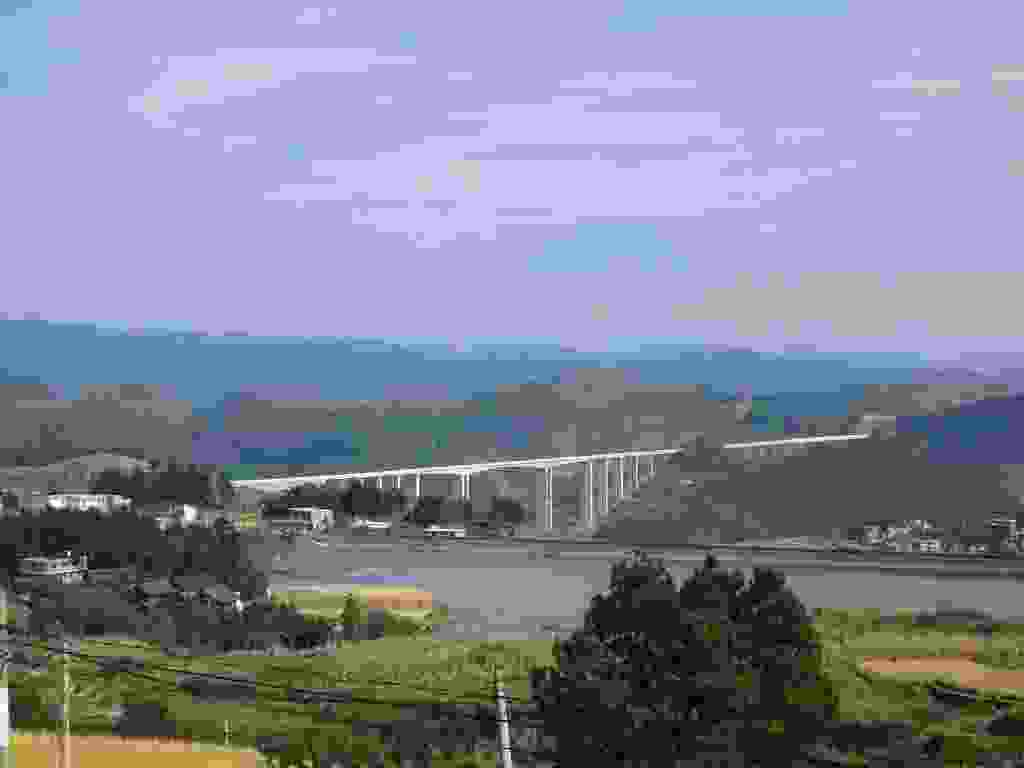
\includegraphics[height=90mm]{../wp-content/uploads/2015/10/PA120196-1024x768.jpg} } 
 \newline
 Régulièrement je croise des cyclistes chinois \newline
 \newline
\centerline{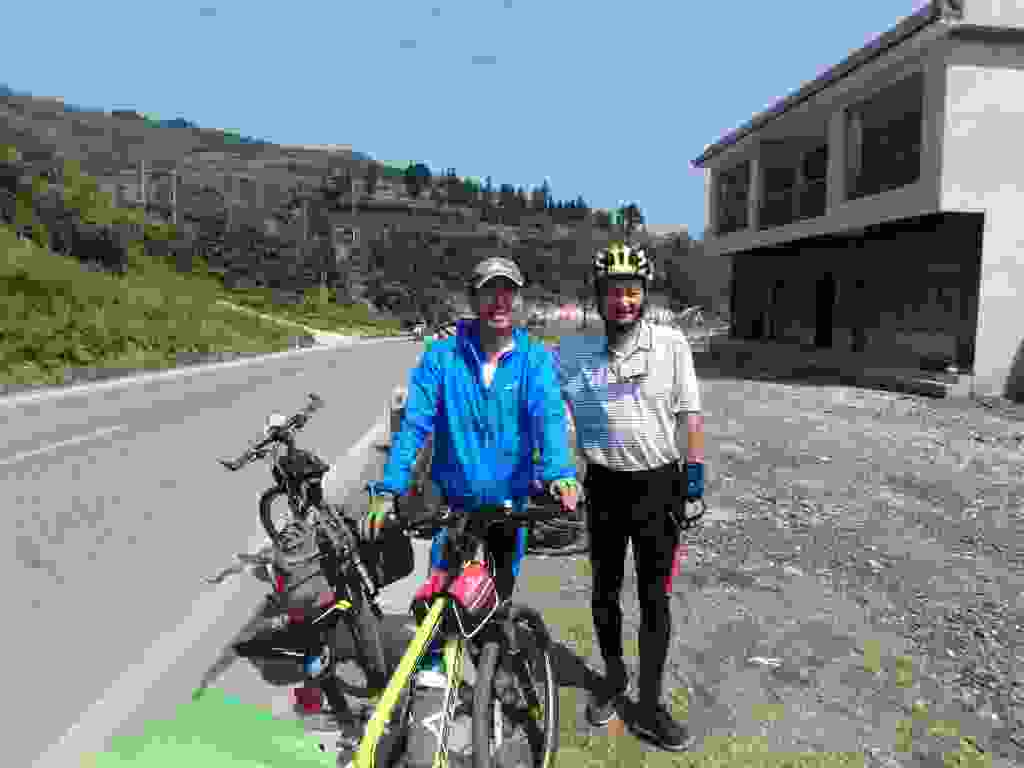
\includegraphics[height=90mm]{../wp-content/uploads/2015/10/PA110184-1024x768.jpg} } 
 \newline
 Même un petit cycliste qui vient échanger quelques mots en anglais \newline
 \newline
\centerline{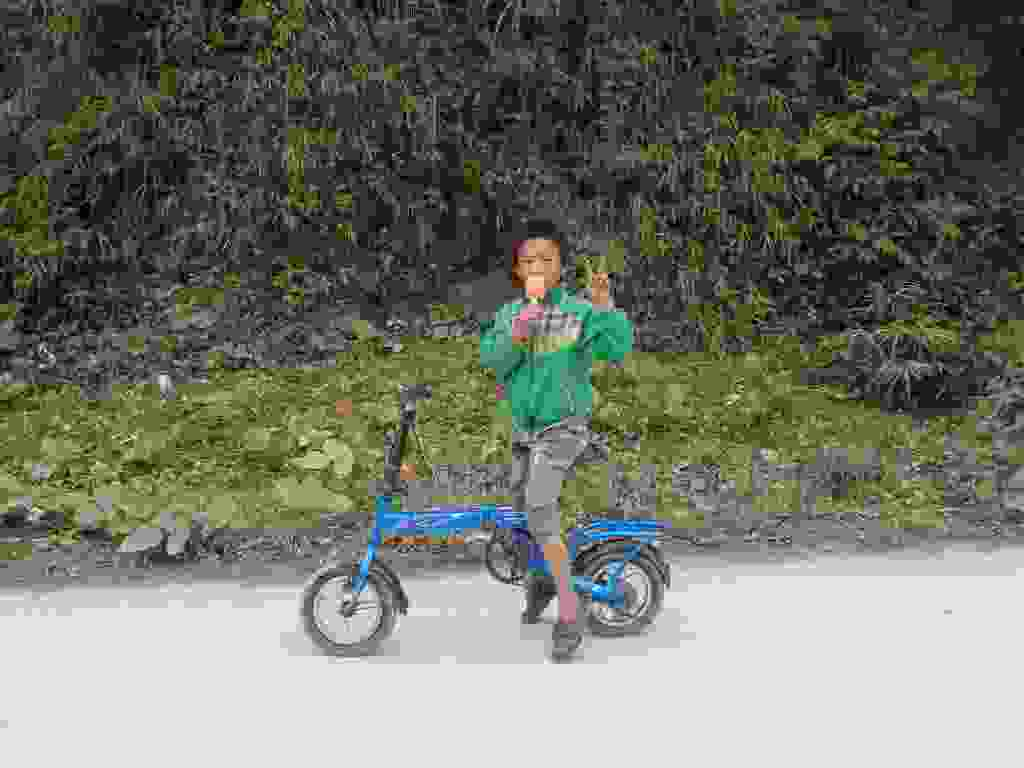
\includegraphics[height=90mm]{../wp-content/uploads/2015/10/PA130209-1024x768.jpg} } 
 \newline
 Je n'ai pas testé ce restaurant \newline
 \newline
\centerline{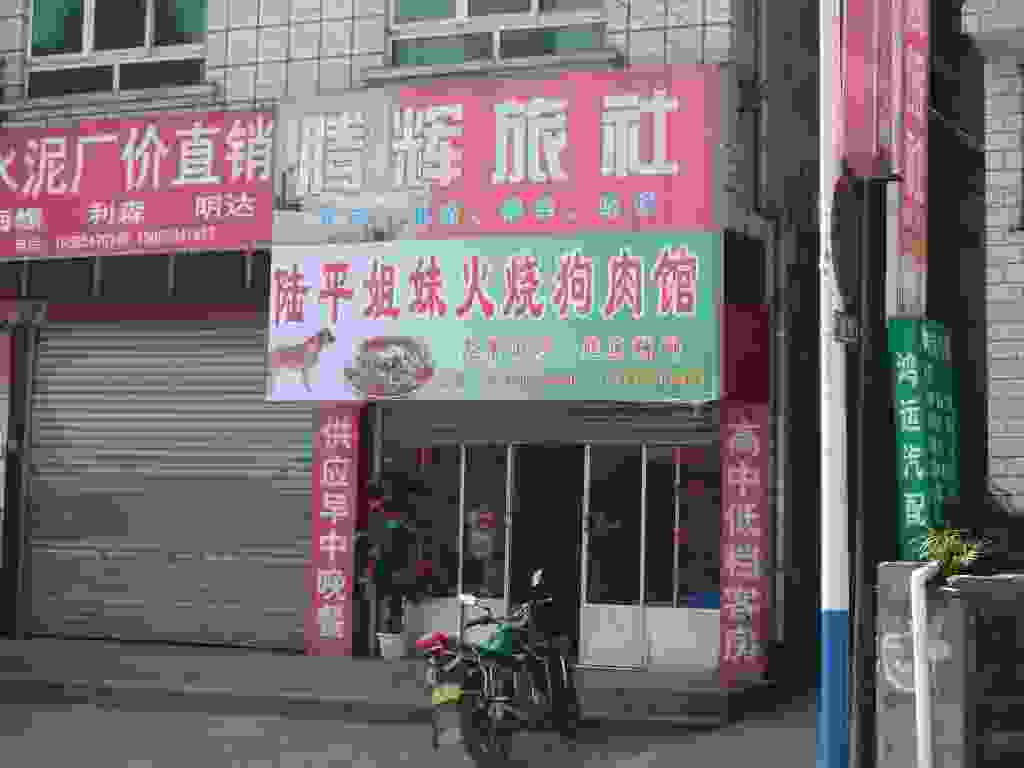
\includegraphics[height=90mm]{../wp-content/uploads/2015/10/PA110186-1024x768.jpg} } 
 \newline
 J'entre dans une partie du Guizhou peuplée par des minorités ethniques. \newline
 \newline
\centerline{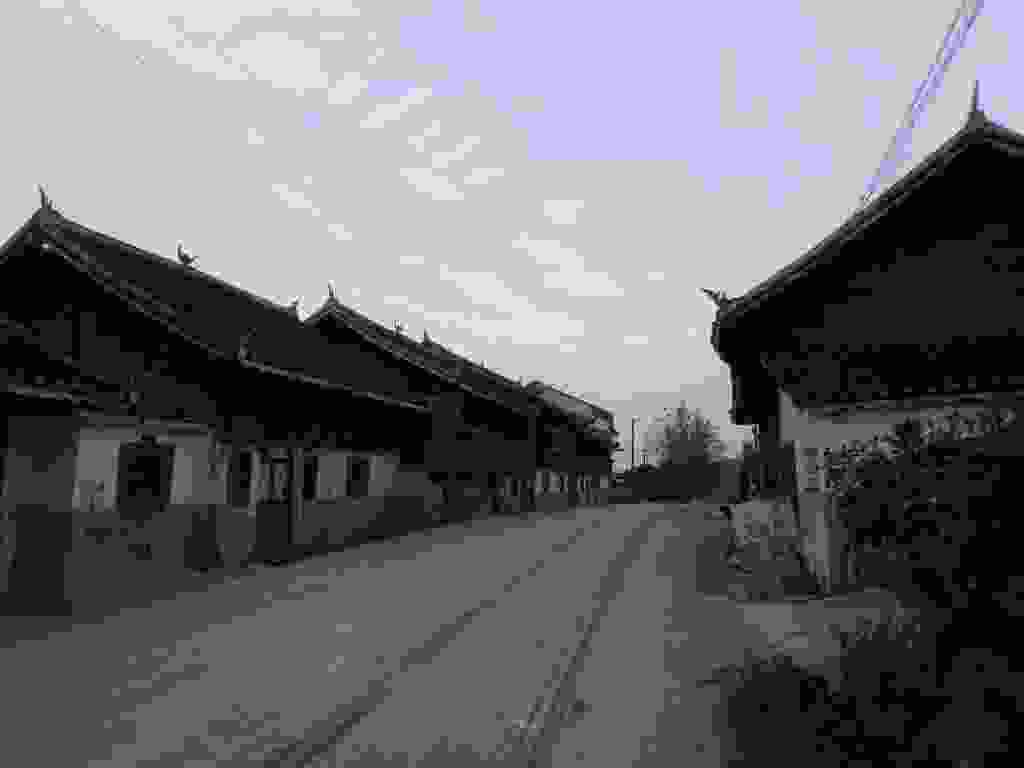
\includegraphics[height=90mm]{../wp-content/uploads/2015/10/PA130200-1024x768.jpg} } 
 \newline
 \newline
\centerline{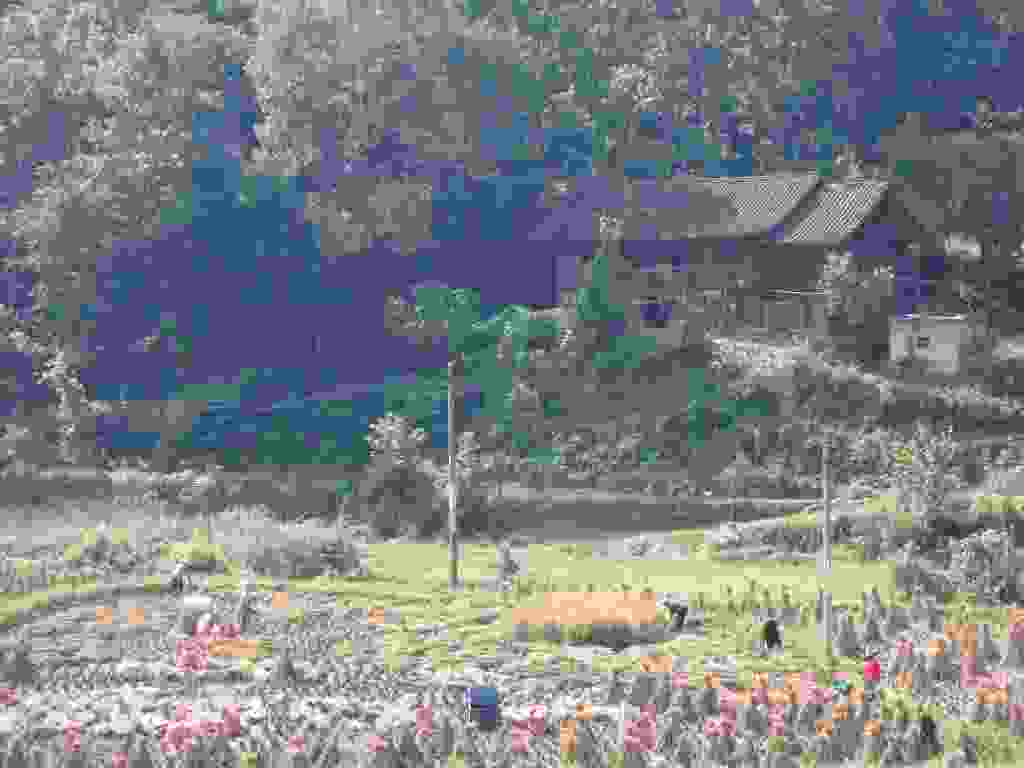
\includegraphics[height=90mm]{../wp-content/uploads/2015/10/PA120191-1024x768.jpg} } 
 \newline
 \newline
\centerline{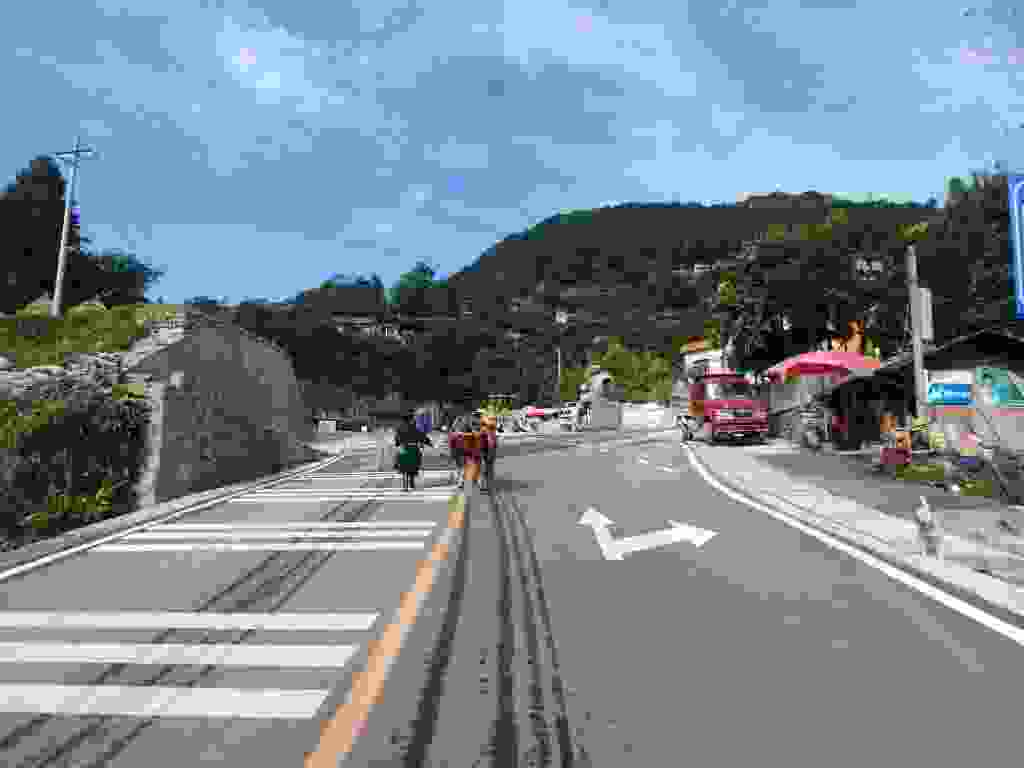
\includegraphics[height=90mm]{../wp-content/uploads/2015/10/PA120193-1024x768.jpg} } 
 \newline
 \newline
\centerline{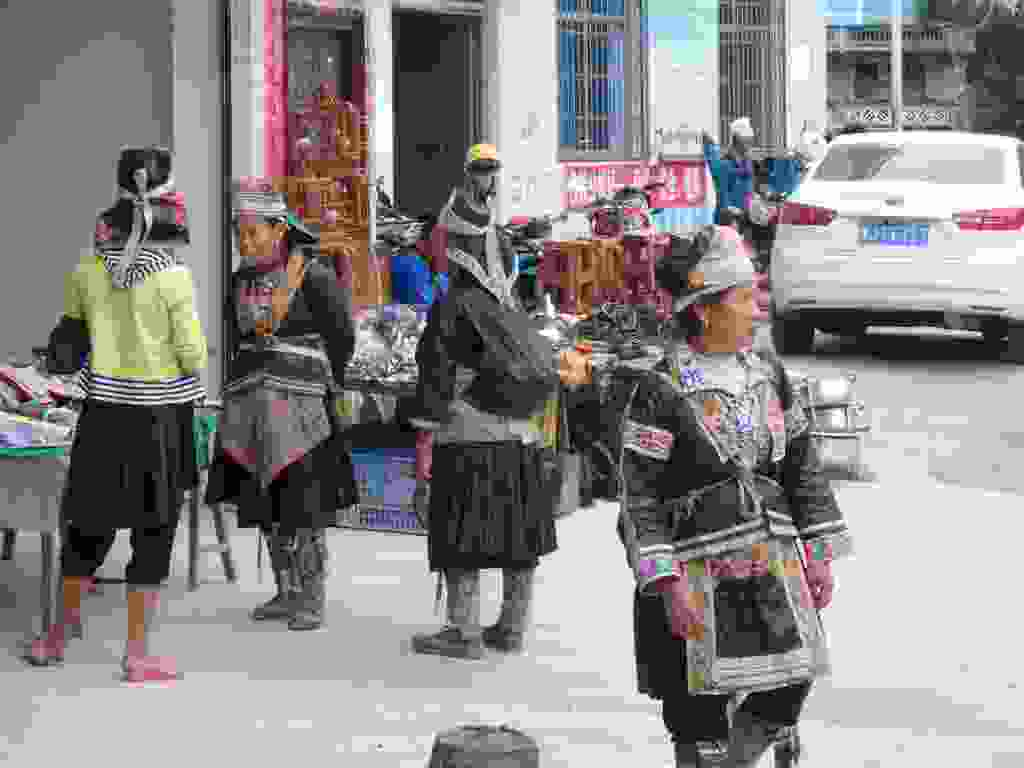
\includegraphics[height=90mm]{../wp-content/uploads/2015/10/PA130208-1024x768.jpg} } 
 \newline
 Sur cette photo noter la position habituelle du chinois qui attend au bord de la route, essayez, moi je ne peux pas y rester… \newline
 \newline
\centerline{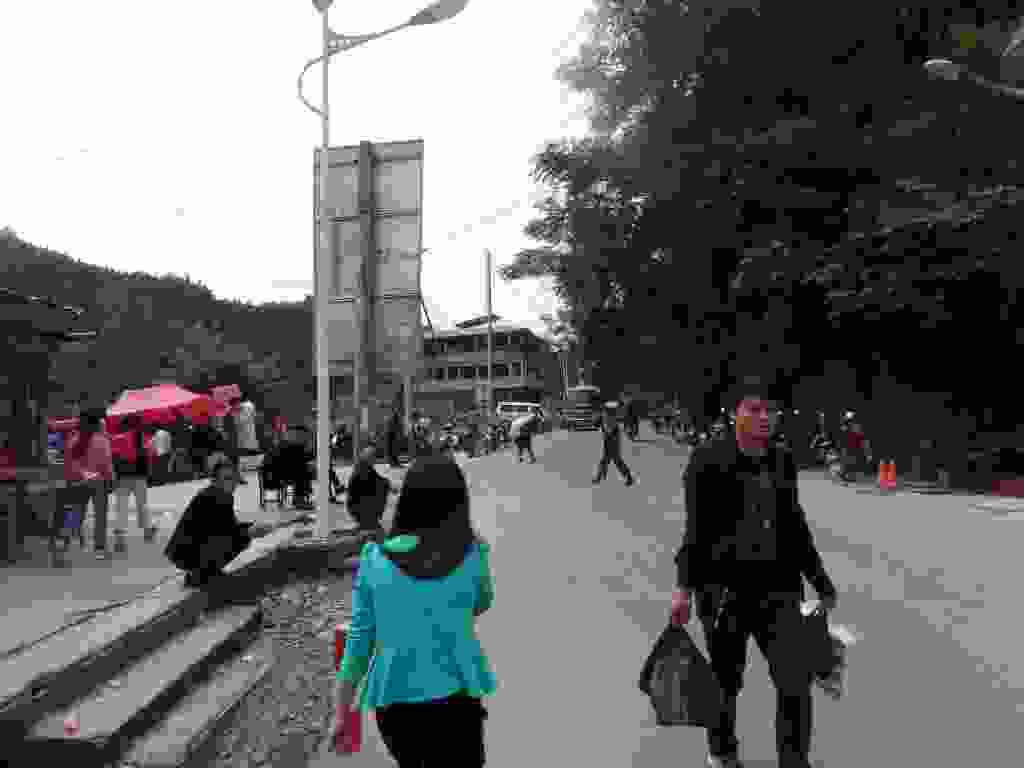
\includegraphics[height=90mm]{../wp-content/uploads/2015/10/PA130204-1024x768.jpg} } 
 \newline

\newpage
 
